\documentclass[a4paper]{book}

% Preambulo por defecto
% Paquetes para usar bien el idioma español
\usepackage[spanish,es-tabla]{babel}
\selectlanguage{spanish}
\usepackage[utf8]{inputenc}

% Paquetes para usar mejores imagenes
\usepackage{graphicx}

% Paquetes para links y tabla de contenidos en el PDF
\usepackage{hyperref}
\hypersetup{colorlinks=true,allcolors=blue}
%\usepackage{hypcap}

% Paquetes para mejores tablas
\usepackage{booktabs}

% Mejor matematica
\usepackage{amsmath}

% Fuentes de las imagenes
\usepackage[absolute,overlay]{textpos}

% Paquete captions
\usepackage[justification=centering,labelformat=empty,labelsep=none]{caption}

% Opciones para ticks
\usepackage{tikz}
\usetikzlibrary{shapes,arrows,positioning}

\tikzstyle{decision} = [diamond, draw, fill=blue!20, text width=4em, text badly centered, node distance=2cm, inner sep=0pt,on grid]
\tikzstyle{block} = [rectangle, draw, fill=blue!20, text width=8em, text centered, rounded corners, minimum height=2em,on grid]
\tikzstyle{line} = [draw, -latex]

% Citas bibliograficas
\usepackage[backend=biber]{biblatex}
\renewcommand{\footnotesize}{\tiny}
\addbibresource{biblio.bib}

% Mejoro las captions
\setbeamertemplate{caption}{\raggedright\insertcaption\par}

\setbeamertemplate{caption}{%
\begin{beamercolorbox}[wd=0.85\paperwidth, sep=.2ex]{block body}\insertcaption%
\end{beamercolorbox}%
}


% Sacar barra de navegacion
\setbeamertemplate{navigation symbols}{}%remove navigation symbols

% Transparencias en items
\setbeamercovered{transparent}

% Estilo de diapositivas
% \usetheme{Boadilla}
\usecolortheme{whale}
\usecolortheme{orchid}

\usepackage{fancyvrb}
% Ejemplos, observaciones y teorema
\theoremstyle{definition}
\newtheorem{exa}{Ejemplo}[section]
\newtheorem{obs}{Observación}[section]
\newtheorem{act}{Actividad}[section]


% Referencias menu
\newtoggle{FirstOne}%
\newcommand*{\menu}[1]{%
\toggletrue{FirstOne}%
\foreach \x in {#1} {%
\iftoggle{FirstOne}{}{${}\rightarrow{}$}
\emph{\x}%
\global\togglefalse{FirstOne}%
}%
}%

% Referencias archivo
\newtoggle{SecondOne}%
\newcommand*{\file}[1]{%
\toggletrue{SecondOne}%
\foreach \x in {#1} {%
\iftoggle{SecondOne}{}{${}/{}$}%
\texttt{\x}%
\global\togglefalse{SecondOne}%
}%
}%

\usepackage{emptypage}


\title{{Nivel 2: Herramientas de teledetecci\'on cuantitativa}\\
\emph{Gu\'{\i}a de actividades: Uso del suelo en el departamento de Iguaz\'u,
provincia de Misiones}}
\date{2017-1}
\author{Francisco Nemiña\thanks{\texttt{fnemina@conae.gov.ar}}}
\affil{Unidad de Educacion y Formacion Masiva \\ Comisi\'on Nacional de Actividades Espaciales}

\graphicspath{{./figs/}}



\begin{document}
\frontmatter
\maketitle

\tableofcontents

\chapter{Introducción}
\label{sec:intro}

La utilización de imágenes satelitales permite analizar grandes extensiones del
territorio, contando con un registro histórico con el cual realizar
comparaciones.

En la provincia de Misiones, el departamento de Iguaz\'u es lindante a Brasil y
Paraguay siendo parte de la zona conocida como triple frontera
perteneciente a la ecorregi\'on conocida como \emph{selva paranaense} (Figura \ref{parque}). All\'i podemos encontrar Represa de Urugua-\'{\i} y el Parque Nacional
Iguaz\'u. El departamento tiene un area de $2.736 km^2$ y una poblaci\'on de
$82.227$ seg\'un el \'ultimo senso del INDEC.

\begin{figure}[h!]
  \centering
  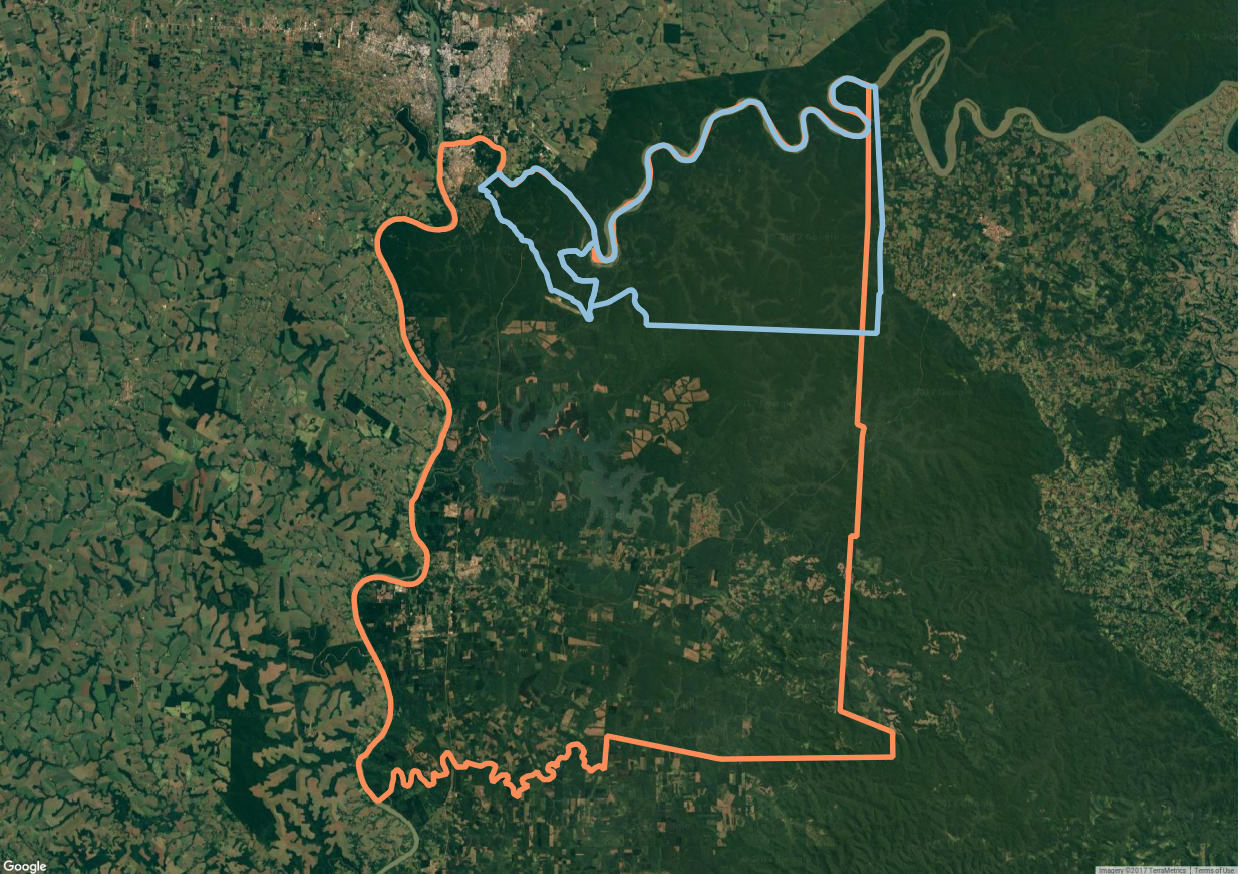
\includegraphics[width=0.8\textwidth]{triple.png}
  \caption{Departamento de Iguaz\'u, en rosa, y parque natural Iguaz\'u, en celeste.}
  \label{parque}
\end{figure}

Tomaremos al departamento como \'area de estudio durante este curso
con el objetivo de obtener un mapa de uso y cobertura que nos
permita estimar y validar sus superficies.

Utilizaremos imagenes de los satelites Landsat 8, Landsat 7 y
el producto de MOD13Q1 obtenido de los satelites TERRA y AQUA durante
el periodo 2000-2016.

\section{Organizacion del curso}

El curso se divide en dos partes. En la primera trabajaremos con la compresi\'on
del espacio espectral y el uso de las im\'agenes satelitales para extraer valores continuos de las variables biof\'isicas.

Cap\'itulo  \ref{viaje}, \nameref{viaje}, estudiaremos las firmas espectrales de
distintas coberturas y como se relacionan con las propiedades biofisicas.
Introduciremos el concepto de espacio espectral como el
lugar natural donde realizar el an\'alisis en teledetecci\'on.

Cap\'itulo  \ref{rebotando}, \nameref{rebotando}, estudiaremos distintas
formas de obtener la reflectancia de las coberturas a partir de los datos satelitales. Analizaremos m\'etodos de correcci\'on atmosf\'erica basados en propiedades estad\'isticas de las im\'agenes y en el modelado de la atm\'osfera.

Cap\'itulo  \ref{abaco}, \nameref{abaco}, veremos como a partir de los valores de reflectancia para una cobertura y operaciones matem\'aticas, podemos obtener los valores de variables biof\'isicas continuas como son el contenido de clorofila o humedad.

Cap\'itulo  \ref{rotaciones}, \nameref{rotaciones}, empezaremos a utilizar herramientas geom\'etricas en el espacio espectral para resaltar distintas propiedades de las im\'agenes y poner en evidencia cuales son las zonas del espectro que m\'as informaci\'on aportan sobre nuesta zona de estudio.

En la segunda parte del curso trabajaremos m\'as en detalle con el espacio
espectral usando sus propiedades para extraer informaci\'on categ\'orica de
las im\'agenes.

Cap\'itulo  \ref{otrolado}, \nameref{otrolado}, veremos como utilizar herramientas que no requieren de conocimiento previo del \'area de estudio para realizar segmentaciones en el espacio de fases de la imagen y obtener mapas de uso y cobertura.

Cap\'itulo  \ref{educando}, \nameref{educando}, veremos otros m\'etodos para extraer informaci\'on categ\'orica sobre las im\'agenes satelitales al estudiar distintas formas de clasificaci\'on supervisada.

Cap\'itulo  \ref{pos}, \nameref{pos}, veremos algunas t\'ecnicas de postprocesamiento que nos permitiran analizar el contexto espacial de nuestras clasificaciones y calcular superficies de coberturas para las im\'agenes y su correspondiente incerteza.

Puede consultar el cronograma detallado en el apendice \ref{chap:cronograma}.

\subsection{Forma de aprobaci\'on}
Para aprobar el curso se deben reunior al menos 100 puntos entre las distintas actividades. Adem\'a deberan completarse dos cuestionarios \emph{obligatorios} al comenzar y finalizar el curso.

La nota final del curso estara dada por el siguiente rango

\begin{itemize}
\item 0 - 99 - No aprobó
\item 100-109 - Seis
\item 110-129 - Siete
\item 130-169 - Ocho
\item 170-189 - Nueve
\item 190-200 - Diez
\end{itemize}

Los puntos se determinan de la siguiente manera

\begin{itemize}
  \item Cada cuestionario: 0 a 10 puntos. Máximo 70.
  \item Cada tarea: 0 a 50 puntos. Máximo 100.
  \item Participar en la plataforma: 0 a 10 puntos. Sin máximo.
\end{itemize}

\section{Material del curso}
Todo el material del curso se encuentra disponible para descargar en el aula virtual del curso. Est\'a organizado de la siguiente manera

\dirtree{%
    .1 material.
    .2 aux\_data.
    .2 example\_scripts.
    .2 raster\_data.
    .2 vector\_data.
    }

conteniendo la carpeta \file{aux\_data} archivos adicionales para trabajar, \file{example\_scripts} todos los scripts que se encuentran en esta guia, \file{raster\_data} los archivos raster cada uno en una carpeta y \file{vector\_data} los archivos vectoriales para usar durante el curso.

Todos los materiales del curso, con sus correspondientes editables, pueden
encontrarse en el repositorio de github \url{https://github.com/fnemina/curso-sopi-herramientas-cuantitativas}.

\mainmatter

\part{Variables continuas}

\chapter{Un viaje del sol a los p\'ixeles.}
\label{viaje}
En esta primera práctica nos familiarizaremos con las interfaces gráficas del
QGIS y de R-studio analizando la imagen Landsat 8 de noviembre de
2016, desde el punto de vista espectral. Son nuestros objetivos:

\begin{itemize}
    \item Abrir una imagen en QGIS.
    \item Crear archivos vectoriales y digitalizar coberturas en QGIS.
    \item Abrir un archivo raster y vectorial en R.
    \item Realizar un análisis estad\'istico de la imagen y de las
        distintas coberturas digitalizadas en R.
\end{itemize}
\section{Exploración de im\'agenes con el QGIS}

Comenzamos abriendo la imagen \file{LC82240782016304LGN00.vrt} que se encuentra
en la carpeta \file{raster\_data,LC82240782016304}, la cual  corresponde al
departamento de Iguaz\'u en la provincia de Misiones. Fue obtenida por
el satelite Landsat 8 durante el mes de noviembre de 2016.

En el menú \menu{Capa, Añadir capa, Añadir capa ráster}. Navegamos
hasta la carpeta \file{raster\_data/LC8224078201630} y abrimos la imagen
\file{LC82240782016304LGN00.vrt}. La encontraremos
en el \menu{Panel de capas} de QGIS. Podemos usar las herramientas para
movernos en la imagen (Figura \ref{fig:move}).

\begin{figure}[h!]
\begin{center}
    
\includegraphics[scale=0.5]{move.png}
\end{center}
\caption{Herramientas para moverse dentro de la imagen. De izquierda a derecha:
    1. Desplazar mapa, 2. Desplazar mapa a la selecci\'on, 3. Acercar zoom, 4.
    Alejar zoom, 5. zoom a la resolucion nativa, 6. zoom general, 7. zoom a la
    selecci\'on, 8. zoom a la capa, 9. zoom anterior, 10. zoom siguiente, 11.
    Actualizar.}
\label{fig:move}
\end{figure}

Para realizar cambios en la visualizaci\'on y explorar las propiedades de una
capa, hacemos click derecho sobre ella y luego seleccionamos la opci\'on
\menu{Propiedades}. All\'i podemos ir a la pestaña
\menu{General} para ver datos como el nombre de la capa\footnote{Es un buen
momento para ponerle uno mas sencillo}, la cantidad de filas y columnas del
archivo, el valor digital no v\'alido, el sistema de coordenadas
entre otros (Figura \ref{fig:general}).

\begin{figure}[h!]
\begin{center}
    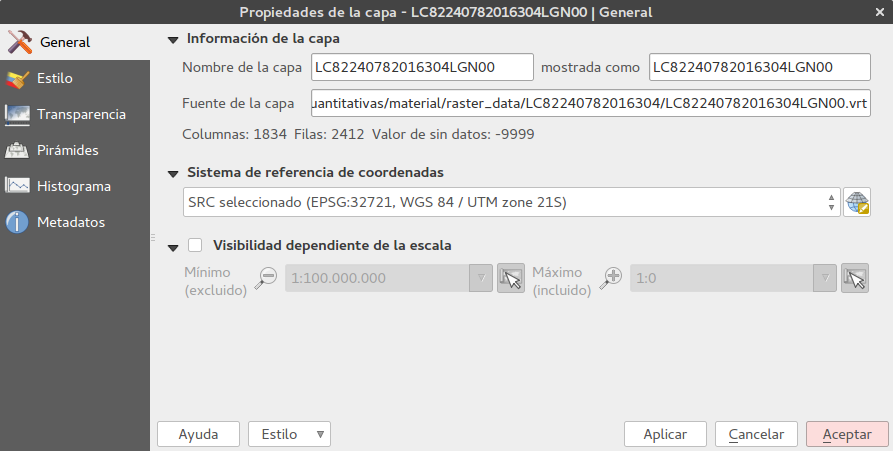
\includegraphics[scale=0.4]{general.png}
\end{center}
\caption{Pestaña general de propiedades de una capa. Podemos ver
    los datos m\'as importantes como la cantidad de filas y
    columnas, el nombre y el sistema de referencia.}
\label{fig:general}
\end{figure}

En la pestaña \menu{Estilo} podemos cambiar la visualizaci\'on de
la capa. All\'i elegimos de que color mostrar cada una de las
bandas. Para cambiar el realce hacemos
click en el boton \menu{Cargar} para seleccionar los valores m\'aximos y m\'inimos
(Figura \ref{fig:estilo}).

\begin{figure}[h!]
\begin{center}
    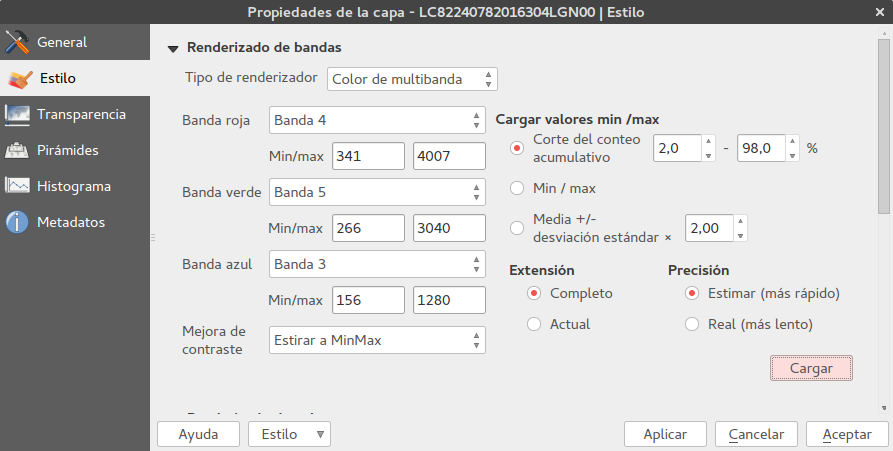
\includegraphics[scale=0.4]{estilo.png}
\end{center}
\caption{Estilos de visualizaci\'on de una capa raster.}
\label{fig:estilo}
\end{figure}

La herramienta \menu{Identificar un objeto espacial} nos permite extraer valores
de la imagen. Al habilitarla veremos datos como el valor
de reflectancia del p\'ixel seleccionado que pueden mostrarse como
\'Arbol, Tabla o Grafo seg\'un uno desee (Figura \ref{fig:grafo}).

\begin{figure}[h!]
\begin{center}
    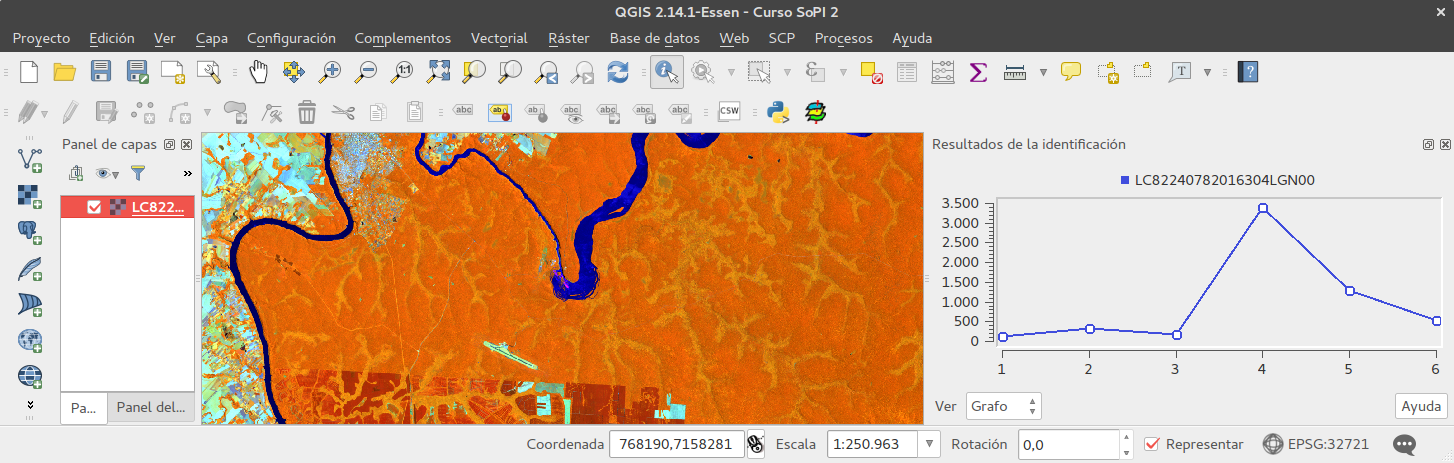
\includegraphics[scale=0.2]{grafo.png}
\end{center}
\caption{Identificaci\'on de un p\'ixel correspondiente a la selva paranaense
    mostrada como grafo. }
\label{fig:grafo}
\end{figure}

\begin{act}
    Cambie la combinación de bandas de la imagen Landsat 8 a color real y expl\'orela.
    Identifique zonas de coberturas uniformes. Pruebe cambiar de
    combinaci\'on de bandas y decida si las zonas siguen siendo uniformes
    despu\'es de cada cambio.
\end{act}

\begin{act}
    Encuentre el sistema de coordenadas en el cual se obtenga la imagen.
    ¿Cu\'antas filas y columnas tiene?
\end{act}

\begin{act}
   Utilizando la herramienta identificar objetos espaciales encuentre los
   valores de reflectancia de distintas coberturas. Grafique estos  valores en
   funci\'on de la longitud de onda y en el espacio espectral.
\end{act}

\section{Creaci\'on de capas vectoriales}

La capas vectoriales nos ser\'a de utilidad en este curso, para extrar datos
cuantitativos de las capas raster.

Con la herramienta \menu{nueva capa de archivo shape} es posible crear una nueva
capa vectorial. Para esto hacemos click en el bot\'on que se
encuentra en el panel lateral. Podemos agregar los campos que sean necesarios
para nuestra capa vectorial. En este caso, ser\'an los campos: MC\_ID, como
entero de longitud 1 y Comment, como texto de 80 caracteres. Elegimos el sistema
de coordenadas correspondiente a la imagen anterior, guardamos en la carpeta
\file{vector\_data/}, con el nombre \file{firmas.shp} (Figura \ref{fig:newshape}).

\begin{figure}[h!]
\begin{center}
    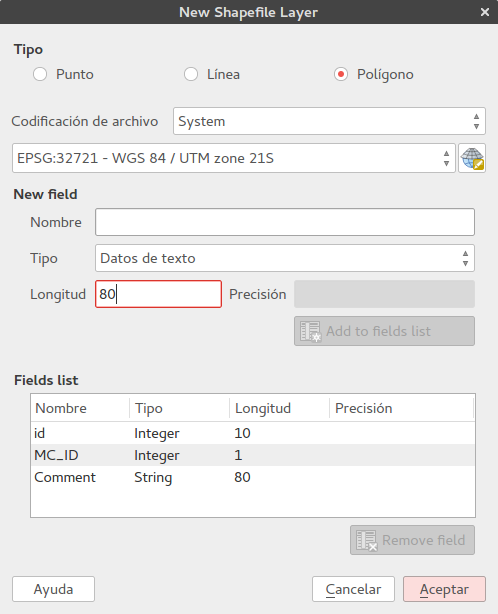
\includegraphics[scale=0.4]{new_shape.png}
\end{center}
\caption{Creaci\'on de una nueva capa vectorial.}
\label{fig:newshape}
\end{figure}


Una vez creada, utilizamos la barra de herramientas de QGIS, (Figura \ref{fig:shapetool}),
para agregarle geometr\'ias. Para esto hacemos click en el bot\'on
de agregar geometr\'ia y digitalizamos una zona uniforme dentro de la imagen.
\begin{figure}[h!]
\begin{center}
    
\includegraphics[scale=0.5]{shapetool.png}
\end{center}
\caption{Herramientas de edición vectorial. De izquierda a derecha: 1. Conmutar
    edici\'on, 2. Guardar cambios a la capa, 3. Añadir objeto espacial, 4. Añadir
    cadena circular, 5. Mover objeto espacial, 6. Herramienta de nodos, 7.
    Borrar lo seleccionado, 8. Cortar objetos espaciales, 9. Copiar objetos
    espaciales, 10. Pegar objetos espaciales.}
\label{fig:shapetool}
\end{figure}

Al terminar, QGIS pedir\'a un n\'umero de ID para la capa que debe ser
correlativo. Además podremos ingresar en este momento los valores del resto de
los campos de nuestro objeto espacial (Figura \ref{fig:newpoli}).

\begin{figure}[h!]
\begin{center}
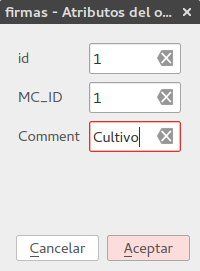
\includegraphics[scale=0.4]{new_poli.png}
\end{center}
\caption{Valores de los campos del nuevo poligono creado.}
\label{fig:newpoli}
\end{figure}

Es importante recordar que debemos estar en el modo de edici\'on para poder hacerlo.
Al terminar debemos desactivar esa opci\'on.

\begin{act}
   Digitalice coberturas uniformes dentro de la imagen. Recuerde obtener al
   menos un pol\'igono por cada categor\'ia de uso y cobertura presente.
\end{act}

En caso de necesitar cambiar la visualizaci\'on de la capa vectorial, podemos entrar
a sus propiedades\footnote{Pueded utilizar el estilo precargado
ubicado en la carpeta \file{aux\_data}}. Podemos acceder a la tabla de
datos de la capa vectorial haciendo click derecho sobre ella y eligiendo la
opci\'on \menu{Abrir tabla de atributos}.

\section{Exploraci\'on raster en R}

Veamos como abrir y trabajar con las im\'agenes satelitales en R. La forma de
realizar operaciones es escribir comandos en la consola de R-studio y
ejecutarlos presionando enter. Para trabajar con im\'agenes satelitales debemos utilizar
algunas librerias adicionales. Para cargarlas usamos el comando
\texttt{library(raster)}. De esta forma agregamos funciones que nos facilitaran
el trabajo raster.

Adem\'as, deberemos situar nuestra carpeta de trabajo donde se encuentran las
carpetas que descargamos. Para esto nos movemos en el explorador de archivos
hasta ella y hacemos click en usar la carpeta como carpeta de trabajo (Figura \ref{fig:setwd}).

\begin{figure}[h!]
\begin{center}
    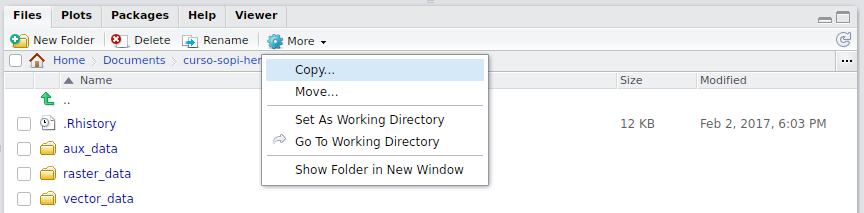
\includegraphics[scale=0.4]{setwd.png}
\end{center}
\caption{Configuraci\'on del directorio de trabajo desde la interfaz gr\'afica.}
\label{fig:setwd}
\end{figure}

Tambi\'en podemos utilizar el comando \texttt{setwd(.)} para configurar el
directorio de trabajo. En este caso hay que especificar la ruta completa hasta
\'el.

Una vez en la carpeta, existen varias maneras de abrir una imagen. Con el comando
\texttt{raster}, abrimos una \'unica banda; \texttt{brick}, abrimos un archivo multibanda,
;y \texttt{stack}, abrimos distintas bandas por separado. Veamos algunos ejemplo:

\begin{exa}
    Abrimos la imagen completa del archivo de Landsat 8 y consultamos sus
    propiedades.
    \begin{lstlisting}
    ref.2016 <- brick("raster_data/LC82240782016304/LC82240782016304LGN00.vrt")
    ref.2016
    \end{lstlisting}
    obtenemos de resultado el siguiente texto
    \begin{Verbatim}[fontsize=\small]
    class       : RasterBrick
    dimensions  : 2412, 1834, 4423608, 6  (nrow, ncol, ncell, nlayers)
    resolution  : 30.00402, 30.00265  (x, y)
    extent      : 731118.6, 786146, 7101531, 7173897  (xmin, xmax, ymin, ymax)
    coord. ref. : +proj=utm +zone=21 +south +datum=WGS84 +units=m +no_defs
                  +ellps=WGS84 +towgs84=0,0,0
    data source : ./material/raster_data/LC82240782016304/LC82240782016304LGN00.vrt
    names       : LC82240782016304LGN00.1, LC82240782016304LGN00.2, ...
    min values  :                     -33,                     192, ...
    max values  :                    2774,                    3265, ...
    \end{Verbatim}
    En \'el, podemos ver la clase a la que corresponde el archivo, en este
    caso un \emph{RasterBrick}, las dimensiones, el tamaño de p\'ixel, extensi\'on
    de la capa, proyecci\'on, cual es la ruta al archivo, las bandas y
    sus valores m\'aximos y m\'inimos.

    Cambiemos el nombre a las bandas y la convertimos a reflectancia entre 0 y 1.

    \begin{lstlisting}
    names(ref.2016) <- c("blue","green","red","nir","swir1","swir2")
    ref.2016 <- ref.2016/1e4
    rasterOptions(addheader = "ENVI")
    writeRaster(ref.2016,"raster\_data/processed/ref2016")
    \end{lstlisting}

    Analicemos el c\'odigo l\'inea por l\'inea.
    \begin{itemize}
    \item La primera abre la imagen como  un raster de m\'ultiples bandas.
    \item La segunda, cambia los nombres de cada banda a los que figuran en la
          lista entre par\'entesis. Es importante resaltar que el n\'umero de nombres
          debe ser el mismo que el de bandas.
    \item En tercer lugar, convertimos el archivo de n\'umeros enteros entre 0 y
          10000 a valores entre 0 y 1.
    \item La cuarta linea es necesaria correrla una sola vez por sesi\'on. La misma
          agrega el header de ENVI a nuestro output para poder abrir el archivo
          desde QGIS
      \item La quinta l\'inea guarda el archivo raster con el nombre \file{ref2016}
          . En este caso estamos usando el formato nativo de R.
    \end{itemize}
    Podemos graficar una combinacion de bandas con el comando
    \texttt{plotRGB(ref.2016,r=4,g=5,b=3, stretch='lin')}(Figura \ref{fig:plot453})

    \begin{figure}[h!]
    \begin{center}
        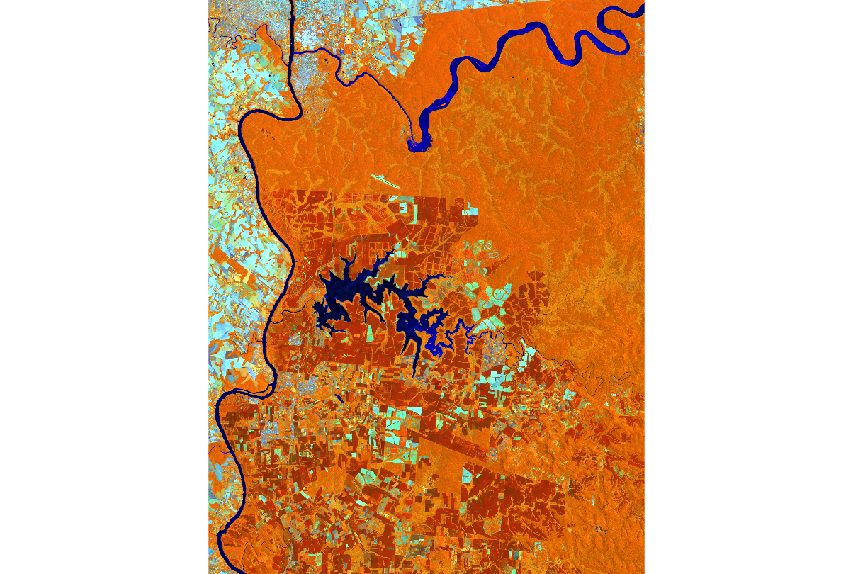
\includegraphics[scale=0.3]{plot453.png}
    \end{center}
    \caption{Combinacion de bandas nir-swir1-red en R.}
    \label{fig:plot453}
    \end{figure}

    Para graficar las bandas por separador hacemos \texttt{plotRGB(ref.2016)}
    (Figura \ref{fig:plotband}).

    \begin{figure}[h!]
    \begin{center}
        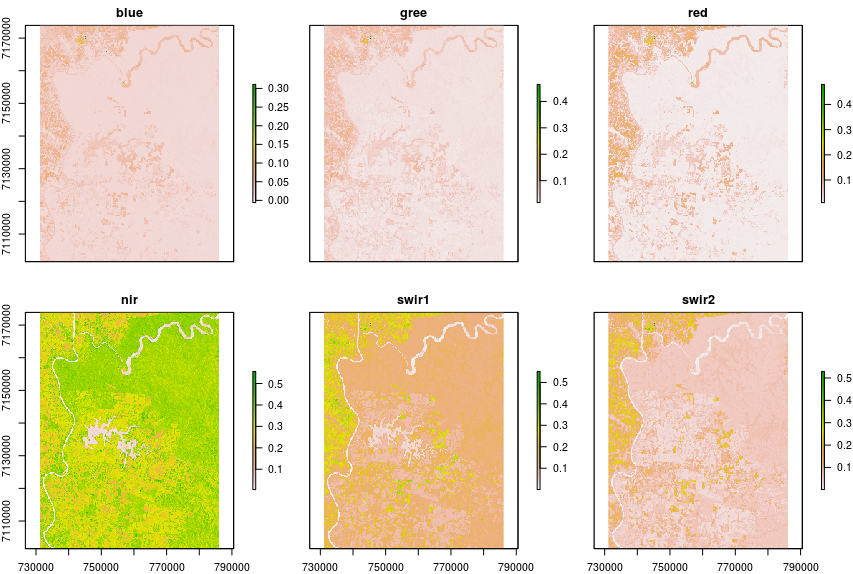
\includegraphics[scale=0.3]{plotband.png}
    \end{center}
    \caption{Gr\'afico de bandas con realce autom\'atico para cada una.}
    \label{fig:plotband}
    \end{figure}

\end{exa}

\begin{act}
   Abra el archivo guardado en QGIS y vuelva a mirar la firma espectral para
   distintas coberturas. ¿Entre que valores se encuentra ahora?
\end{act}

Veamos como trabajar m\'as en detalle con los valores de nuestra imagen.

\begin{exa}

    Hagamos un an\'alisis estad\'istico de la imagen ejecutando el
    comando \texttt{summary(ref.2016)}
    \begin{Verbatim}[fontsize=\small]
               blue   gree    red     nir   swir1   swir2
    Min.    -0.0278 0.0000 0.0000 -0.0128 -0.0069 -0.0038
    1st Qu.  0.0128 0.0328 0.0184  0.2763  0.1198  0.0493
    Median   0.0138 0.0362 0.0203  0.3287  0.1365  0.0572
    3rd Qu.  0.0170 0.0450 0.0329  0.3557  0.1644  0.0749
    Max.     0.5548 0.8257 0.8034  0.7542  0.9181  0.9446
    NA's     0.0000 0.0000 0.0000  0.0000  0.0000  0.0000
    \end{Verbatim}
    Calculamos los histogramas de todas las bandas con el
    comando \texttt{hist(ref.2016)} y el scatter plot entre dos bandas como
  \verb|plot(ref.2016$red,ref.2016$nir)|.

    En caso de querer todos los scatterplots e histogramas en un solo gr\'afico
    usamos el comando \texttt{pairs(ref.2016)}.
    \end{exa}


\section{Manejo vectorial en R}

Hasta ahora estamos analizando la imagen completa, pero podemos analizar
determinadas zonas utilizando un archivo vectorial.. Tambi\'en ser\'a
posible muestrear la imagen usando otro raster, pero lo veremos m\'as adelante.

Para trabajar con vectores en R utilizaremos la libreria
\texttt{library(rgal)}.

\begin{exa}
    Veamos como realizar el an\'alisis b\'asico de un vector en R. Comenzamos
    ley\'endolo

    \begin{lstlisting}
    firmas <- readOGR(dsn="vector\_data/", layer="firmas")
    \end{lstlisting}

    Notamos en este caso que debemos indicar por separado la carpeta que
    contiene al shapefile en \emph{dsn} y el nombre de la capa que queremos
    abrir como \emph{layer}.

    Podemos mostrar las propiedades del vector llamando a la variable
    \texttt{firmas} obteniendo
    \begin{Verbatim}[fontsize=\small]
    class       : SpatialPolygonsDataFrame
    features    : 8
    extent      : 738692.8, 767774.6, 7133396, 7165265  (xmin, xmax, ymin, ymax)
    coord. ref. : +proj=utm +zone=21 +south +datum=WGS84 +units=m +no_defs
                  +ellps=WGS84 +towgs84=0,0,0
    variables   : 3
    names       : id, MC_ID,       Comment
    min values  :  0,     1,          Alto
    max values  :  9,     8, Suelo desnudo
    \end{Verbatim}

    Para graficar los vectores y la imagen juntos hacemos

    \begin{lstlisting}
    plotRGB(ref.2016, stretch="lin")
    plot(firmas,add=TRUE,col='red')
    \end{lstlisting}
    donde la primera l\'inea grafica la imagen de fondo y la segunda agrega el
    shapefile sobre ella.
\end{exa}

\begin{act}
    Muestre las propiedades de la capa raster y vectorial y verifique
    que se encuentren en el mismo sistema de coordenadas.
\end{act}

Veamos como extraer datos de un archivo raster con un vector con la funci\'on
\texttt{extract}. Esta toma dos argumentos, el vector que queremos
utilizar y la capa raster sobre la cual hacer la consulta.

\begin{exa}
    Graficar en un scatterplot de dos bandas mostrando la zona del espacio
    ocupada por una cobertura.
    \begin{lstlisting}
    datos <- extract(ref.2016,firmas)
    \end{lstlisting}
    de esta forma realizamos la extracci\'on de todos los datos de la imagen a una
    lista
    \begin{lstlisting}
    plot(ref.2016$red, ref.2016$nir)
    points(as.data.frame(datos[1])$red, as.data.frame(datos[1])$nir,col="green",
           pch = ".")
    \end{lstlisting}
    Ágregamos el scatterplot al muestreo obteniendo
    \begin{figure}[h!]
    \begin{center}
        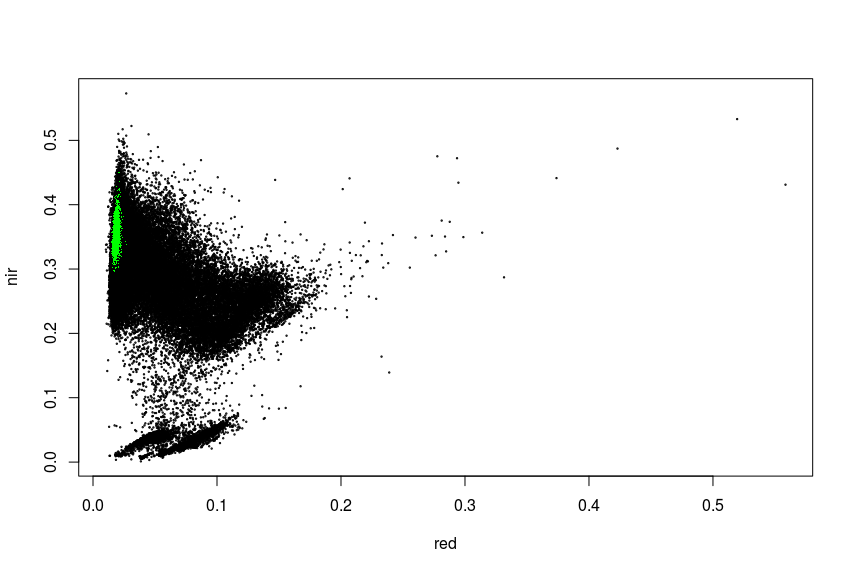
\includegraphics[scale=0.3]{plot-red-nir-zone.png}
    \end{center}
    \caption{Resultado del scatterplot para las bandas roja y nir. Se muestra en
        verde datos correspondientes a la selva paranaense.}
    \label{fig:rednirzone}
    \end{figure}

\end{exa}

La funci\'on \texttt{extract} nos permite tambi\'en aplicar una funci\'on a los datos
extraidos antes de entregarlos al usuario. Veamos como usarla para calcular
datos de interes sobre las coberturas y guardarlo en un archivo vectorial.

\begin{exa}
     Extraer los promedios y desv\'io standar de un raster y agregarlos a un
     vector. Primero extraemos los valores de promedio y desv\'io
     \begin{lstlisting}
     promedio <- extract(ref.2016,firmas,fun=mean)
     desvio <- extract(ref,firmas,fun=sd)
     \end{lstlisting}
     renombramos luego las columnas como promedio y desv\'io seguido de la banda a
     la que pertenecen,
     \begin{lstlisting}
     colnames(promedio) <- paster("mean",colnames("promedio"),sep="_")
     colnames(desvio) <- paster("sd",colnames("desvio"),sep="_")
     \end{lstlisting}
     finalmente agregamos los archivos a un nuevo shapefile
     \begin{lstlisting}
     firmas@data <- cbind(firmas@data,promedio,desvio)
     writeOGR(firmas, sdn="vector_data/processed","firmas_datos",
              driver="ESRI Shapefile")
     \end{lstlisting}
\end{exa}

Finalmente, veamos como usar una capa vectorial para graficar las
firmas espectrales y graficarlas para distintas coberturas

\begin{exa}
     Graficar las firmas espectrales en funci\'on de la longitud de onda para cada
     pol\'igono. Utilizaremos dos nuevas librerias,
     \texttt{reshape2} y \texttt{lattice}

     Comenzamos convirtiendo en dataframe a nuestros promedios, donde cada
     columna corresponde a una firma espectral
     \begin{lstlisting}
     df <- t(promedio)
     colnames(df) <- vector@data$Comment
     \end{lstlisting}
     Agregamos luego una columna con las longitudes de onda en nanometros. Luego
     reformamos el dataframe para que podamos subsetearlo, poniendo finalmente
     los nombres a cada columna
     \begin{lstlisting}
     df$wl <- as.matrix(c(485,560,660,830,1650,2215))
     df <- melt(df,id.vars="wl", variable.name="cobertura")
     names(df) <- c("wl","Cobertura","Reflectancia")
     \end{lstlisting}
     El dataframe resultante deber\'ia ser:
     \begin{Verbatim}[fontsize=\small]
          wl     Cobertura Reflectancia
     1   485          Alto  0.012926561
     2   560          Alto  0.034730646
     3   660          Alto  0.018491884
     4   830          Alto  0.354564681
     5  1650          Alto  0.133750642
     ...
     \end{Verbatim}
     Repetimos el proceso para el desv\'io standar
     \begin{lstlisting}
     dfd <- t(desvio)
     colnames(dfd) <- vector@data$Comment
     dfd$wl <- as.matrix(c(485,560,660,830,1650,2215))
     dfd <- melt("wl","Cobertura","Desvio")
     df$desvio <- dfd$desvio
     df$MC_ID <- as.character(vector@data$MC_ID[match(df$Cobertura,
                              vector@data$Comment)])
     \end{lstlisting}
     El resultado ser\'a ahora
     \begin{Verbatim}[fontsize=\small]
          wl     Cobertura Reflectancia       Desvio
     1   485          Alto  0.012926561 0.0007772473
     2   560          Alto  0.034730646 0.0018113004
     3   660          Alto  0.018491884 0.0011561294
     4   830          Alto  0.354564681 0.0166801398
     5  1650          Alto  0.133750642 0.0075157929
     ...
     \end{Verbatim}
     En primer lugar pondremos todas las firmas espectrales juntas, separadas
     por color, con la libreria \texttt{lattice}
     \begin{lstlisting}
     xyplot(Reflectancia~wl, data=df, groups = Cobertura,
            auto.key=list(space="top", columns=4),
            ty=c("l", "p"))
     \end{lstlisting}
     Aqu\'i la primer l\'inea dice que grafiquemos la reflectancia como funci\'on de
     la longitud de onda, obteniendo los datos del dataframe DF y agrupandolos
     seg\'un la columna cobertura. La siguiente l\'inea agrega la leyenda en la
     parte superior de la figura con 4 columnas. Por \'ultimo en la tercer l\'inea
     pedimos que el gr\'afico tenga l\'ineas y puntos (Figura \ref{fig:spectra-1}).

     \begin{figure}[h!]
     \begin{center}
         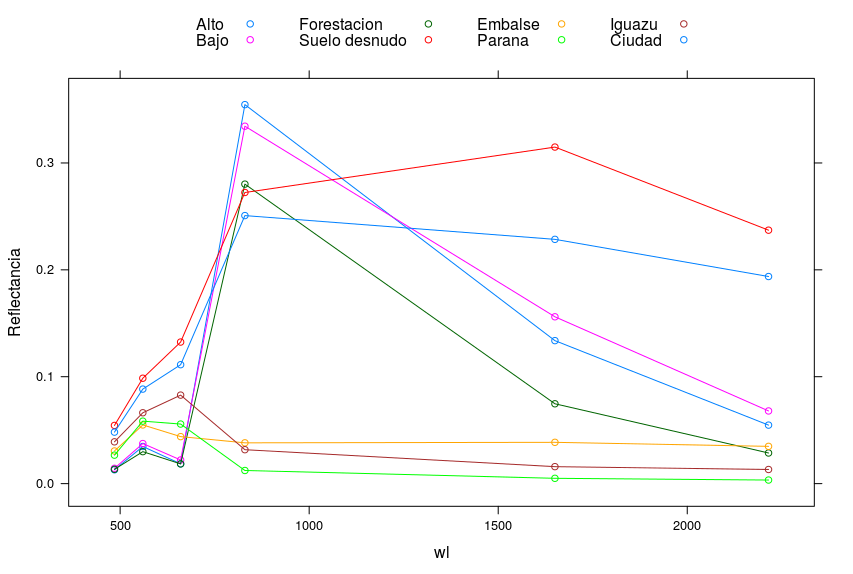
\includegraphics[scale=0.3]{spectra-1.png}
     \end{center}
     \caption{Firmas espectrales}
     \label{fig:spectra-1}
     \end{figure}

     Si queremos agruparlo por categor\'ia de uso y cobertura cambiamos la formula
     \texttt{Reflectancia ~ wl} por \texttt{Reflectancia \~ wl | MC\_ID}
     \begin{lstlisting}
     xyplot(Reflectancia ~ wl | MC_ID, data=df, groups = Cobertura,
            auto.key=list(space="top", columns=4),
            ty=c("l", "p"))
     \end{lstlisting}

     Si queremos graficar solo un subset de datos (Figura \ref{fig:spectra-2}).

     \begin{lstlisting}
     xyplot(Reflectancia~wl | MC_ID, data=df, groups = Cobertura,
            auto.key=list(space="top", columns=4), ty=c("l", "p"),
            subset = Cobertura %in% c("Alto","Bajo"))
     \end{lstlisting}
     \begin{figure}[h!]
     \begin{center}
         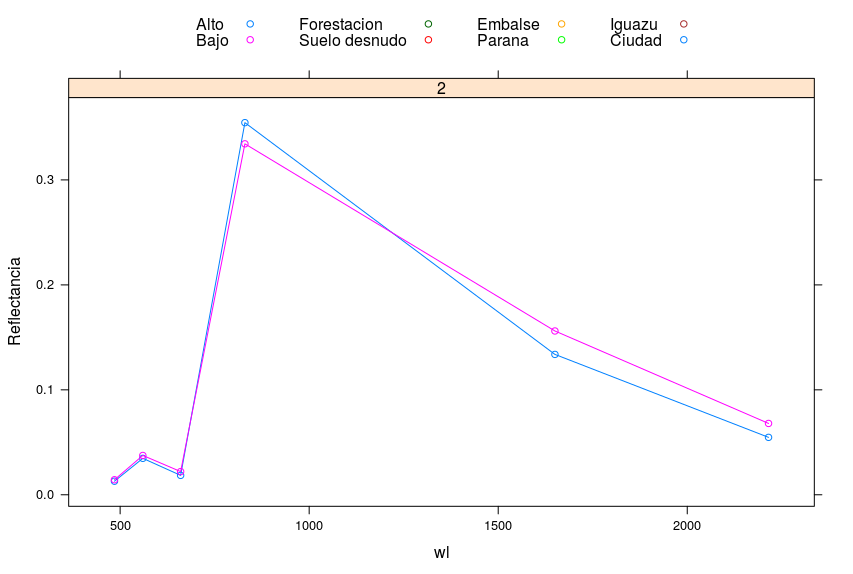
\includegraphics[scale=0.3]{spectra-2.png}
     \end{center}
     \caption{Firmas espectrales}
     \label{fig:spectra-2}
     \end{figure}
 \end{exa}

\begin{act}
    Grafique la media y el desv\'io standar para las distintas coberturas que pudo
     identificar en el punto uno.
\end{act}


\chapter{Rebotando por la atm\'osfera}
\label{rebotando}

En esta segunda actividad pr\'actica nos centraremos en la correcci\'on radiom\'etrica
de im\'agenes satelitales. Son nuestros objetivos:

\begin{itemize}
    \item Abrir una imagen satelital desde el metadato.
    \item Convertir los valores de la imagen a reflectancia a tope de la
        atm\'osfera.
    \item Corregir la imagen satelital utilizando los m\'etodos de \emph{dos} y
        \emph{cost}
    \item Corregir la imagen satelital utilizando el \emph{6S} en su versi\'on web.
\end{itemize}

\section{C\'alculo de reflectancia a tope de la atm\'osfera}

Para poder convertir una imagen a reflectancia a tope de la atm\'osfera vamos a
necesitar la informaci\'on adicional que hallaremos en su metadato.
Para abrirla desde el metadato utilizaremos las funciones
disponibles en la libreria \texttt{RStoolbox}.

\begin{exa}
    Abramos  la imagen Landsat 7
    del año 2000 desde el metadato y la mostraremos en combinaci\'on color real
    y analicemos sus propiedades.
    \begin{lstlisting}
    meta.2000 <- readMeta("raster_data/LE72240782000188EDC00/LE72240782000188EDC00_MTL.txt")
    \end{lstlisting}
    Podemos mostrar las distintas variables incluidas en el objeto usando el
    signo \$ y su nombre. Por ejemplo, \verb|meta.2000$SOLAR_PARAMETERS|
    da como resultado
    \begin{Verbatim}[fontsize=\small]
     azimuth elevation  distance
    37.38251  31.14409   1.01670
    \end{Verbatim}
    Usando el metadato podemos cargar la imagen completa con el comando
    \texttt{stackMeta}. Eliminamos, en este caso, las bandas 6 y 7 por
    ser t\'ermicas.
    \begin{lstlisting}
    dn.2000 <- stackMeta(meta.2000)
    dn.2000 <- dn.2000[[-6:-7,]]
    dn.2000
    \end{lstlisting}
    El resultado es un objeto \emph{raster stack} como el que sigue
    \begin{Verbatim}[fontsize=\small]
    class       : RasterStack
    dimensions  : 2412, 1834, 4423608, 6  (nrow, ncol, ncell, nlayers)
    resolution  : 30.00402, 30.00265  (x, y)
    extent      : 731118.6, 786146, 7101531, 7173897  (xmin, xmax, ymin, ymax)
    coord. ref. : +proj=utm +zone=21 +south +datum=WGS84 +units=m +no_defs
                  +ellps=WGS84 +towgs84=0,0,0
    names       : B1_dn, B2_dn, B3_dn, B4_dn, B5_dn, B7_dn
    min values  :     0,     0,     0,     0,     0,     0
    max values  :   255,   255,   255,   255,   255,   255
    \end{Verbatim}
    Mostramos la imagen en cobinaci\'on color real con \texttt{plotRGB(dn.2000, r=3, g=2, b=1, stretch="lin")}
    (Figura \ref{fig:dn-l7-rgb}).
     \begin{figure}[h!]
     \begin{center}
         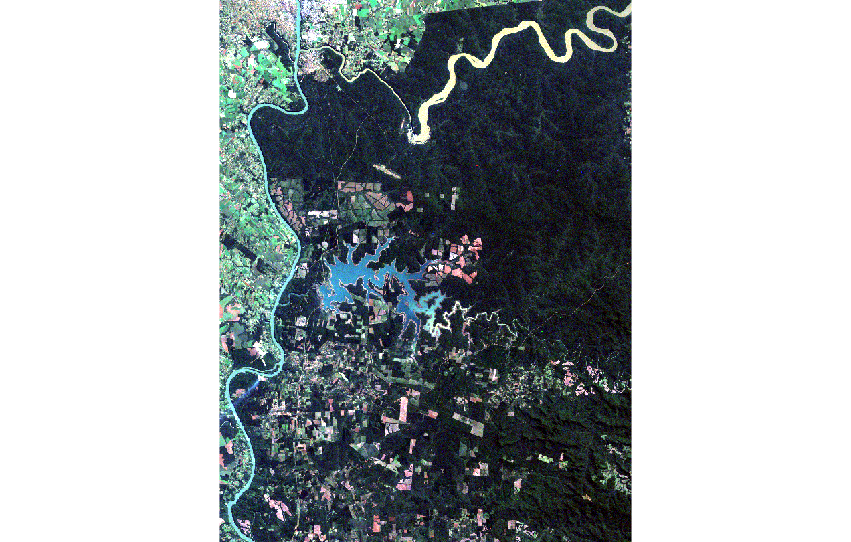
\includegraphics[scale=0.6]{dn-l7-rgb}
     \end{center}
     \caption{Imagen en combinaci\'on de bandas color real de la zona de inter\'es.}
     \label{fig:dn-l7-rgb}
     \end{figure}
\end{exa}

De esta forma tenemos el archivo en n\'umero digital con todos sus metadatos
para convertirlo a reflectancia y realizar las distintas correcciones.

Existen dos formas de convertirla a reflectancia a tope de la atm\'osfera: a mano,
utilizando las herramientas algebraicas de R o con la funci\'on
especifica de \texttt{RStoolbox}.

\begin{exa}
    C\'alculo de reflectancia a tope de la atm\'osfera
    utilizando el metadato paso por paso

    \begin{lstlisting}
    dn2ref.2000 <- meta.2000$CALREF[1:6,]
    elev.2000 <- pi*meta.2000$SOLAR_PARAMETERS['elevation']/180
    \end{lstlisting}
    extraemos primero del metadato los par\'ametros de calibraci\'on en
    reflectancia y el \'angulo de elevaci\'on solar. Convertimos luego la imagen
    a reflectancia y la dividimos por el seno del \'angulo solar.
    Luego cambiamos los nombres de las bandas

    \begin{lstlisting}
    toam.2000 <- (dn.2000*dn2ref.2000$gain+dn2ref.2000$offset)/sin(elev.2000)
    names(toam.2000) <- c("blue","green","red","nir","swir1","swir2")
    \end{lstlisting}

    Otra forma de realizarlo es utilizando la funci\'on
    \texttt{radCor}. En este caso, debemos tener la imagen en DN, el metadato y
    cual es la cantidad que queremos calcular.

    \begin{lstlisting}
    toa.2000 <- radCor(dn.2000, metaData = meta.2000, method = "apref")
    \end{lstlisting}

    Podemos comparar los resultados de ambos m\'etodos inspeccionando los objetos
    \texttt{toam.2000} y \texttt{toa.2000}.
    \begin{Verbatim}[fontsize=\small]
    class       : RasterBrick
    dimensions  : 2412, 1834, 4423608, 6  (nrow, ncol, ncell, nlayers)
    resolution  : 30.00402, 30.00265  (x, y)
    extent      : 731118.6, 786146, 7101531, 7173897  (xmin, xmax, ymin, ymax)
    coord. ref. : +proj=utm +zone=21 +south +datum=WGS84 +units=m +no_defs
                  +ellps=WGS84 +towgs84=0,0,0
    data source : in memory
    names       :        blue,       green,         red,         nir,    swir1,       ...
    min values  : -0.01976113, -0.02181530, -0.02029439,  0.01934678,    -0.02781926, ...
    max values  :   0.6106812,   0.5609009,   0.6079443,   0.8696885,    0.8640919,   ...
    \end{Verbatim}

    y

    \begin{Verbatim}[fontsize=\small]
    class       : RasterStack
    dimensions  : 2412, 1834, 4423608, 6  (nrow, ncol, ncell, nlayers)
    resolution  : 30.00402, 30.00265  (x, y)
    extent      : 731118.6, 786146, 7101531, 7173897  (xmin, xmax, ymin, ymax)
    coord. ref. : +proj=utm +zone=21 +south +datum=WGS84 +units=m +no_defs
                  +ellps=WGS84 +towgs84=0,0,0
    names       :     B1_tre,     B2_tre,     B3_tre,     B4_tre,     B5_tre, ...
    min values  : 0.00000000, 0.00000000, 0.00000000, 0.01934678, 0.00000000, ...
    max values  :  0.6106812,  0.5609009,  0.6079443,  0.8696885,  0.8640919, ...
    \end{Verbatim}

    \end{exa}

\begin{act}
    Inspeccione la reflectancia a tope de la atm\'osfera para todas las bandas.
    Para esto realice los histogramas, graficos de dispersi\'on, calcule la media,
    el desv\'io standar y cualquier otra medida estad\'istica que desee.
\end{act}
\section{C\'alculo de reflectancia corregida atmosf\'ericamente por m\'etodos
            estad\'isticos}

La funci\'on \texttt{radCor} dispone de un par\'ametro para hacer distintos
tipos de correcciones atmosf\'ericas. Ya utilizamos \emph{apref}, que nos permiti\'o
calcular la reflectancia a tope de la atm\'osfera, veamos ahora como aplicar el m\'etodo
de substracci\'on de cuerpo obscuro.

\begin{exa}
    Apliquemos el metodo de \emph{simple dos} para corregir la imagen. En este caso
    solamente restaremos el m\'inimo en cada banda a la imagen para las bandas
    donde existe haze, es decir en la zona del visible y del infrarrojo cercano.

    Estimamos el haze primero y luego corregimos la imagen haciendo
    \begin{lstlisting}
    haze.2000 <- estimateHaze(dn.2000,darkProp = 0.01, hazeBands = 1:4, plot=TRUE)
    sdos.2000 <- radCor(dn.2000, metaData = meta.2000,
                 hazeValues = haze.2000,
                 hazeBands = c("B1_dn","B2_dn","B3_dn","B4_dn"),
                 method="sdos")
    \end{lstlisting}
    en este caso los valores de haze estimados son
    \begin{Verbatim}[fontsize=\small]
    B1_dn B2_dn B3_dn B4_dn
       41    27    20    15
    \end{Verbatim}
    Para hacer un an\'alisis de lo que pasa, vamos a graficar los
    histogramas de cada banda para la imagen en reflectancia TOA y corregida por
    el m\'etodo \emph{simple dos}. Usaremos el paquete \texttt{rasterVis}
    \begin{lstlisting}
    B1 <- densityplot(~B1_tre+B1_sre, data=toa.boa, xlab="Reflectancia",
                      ylab="", main="Banda azul", plot.points=FALSE, xlim=c(0,0.3),
                      key=simpleKey(text=c("Tope de la atmosfera",
                                           "Correccion Simple DOS"),
                                           lines=TRUE, points=FALSE))
    B2 <- densityplot(~B2_tre+B2_sre, data=toa.boa, xlab="Reflectancia",
                      ylab="", main="Banda verde", plot.points=FALSE, xlim=c(0,0.3),
                      key=simpleKey(text=c("Tope de la atmosfera",
                                           "Correccion Simple DOS"),
                                           lines=TRUE, points=FALSE))
    B3 <- densityplot(~B3_tre+B3_sre, data=toa.boa, xlab="Reflectancia",
                      ylab="", main="Banda roja", plot.points=FALSE, xlim=c(0,0.3),
                      key=simpleKey(text=c("Tope de la atmosfera",
                                           "Correccion Simple DOS"),
                                           lines=TRUE, points=FALSE))
    B4 <- densityplot(~B4_tre+B4_sre, data=toa.boa, xlab="Reflectancia",
                      ylab="", main="Banda nir", plot.points=FALSE, xlim=c(0,0.3),
                      key=simpleKey(text=c("Tope de la atmosfera",
                                           "Correccion Simple DOS"),
                                           lines=TRUE, points=FALSE))
     print(B1,split = c(1, 1, 2, 2),more=TRUE)
     print(B2,split = c(2, 1, 2, 2),more=TRUE)
     print(B3,split = c(1, 2, 2, 2),more=TRUE)
     print(B4,split = c(2, 2, 2, 2),more=FALSE)
    \end{lstlisting}
    las primeras 4 funciones crean los histogramas para cada banda
    corregida, mientras que las \'ultimas 4 l\'ineas los imprimen en una grilla (Figura \ref{fig:simpledos}).
    \begin{figure}[h!]
    \begin{center}
        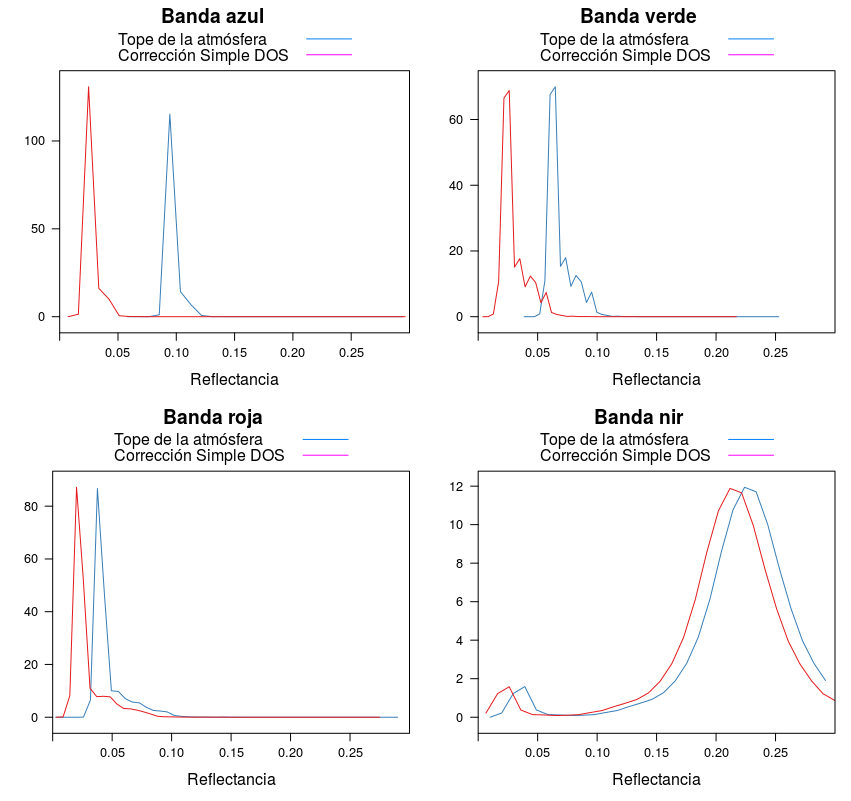
\includegraphics[scale=0.4]{simpledos.png}
    \end{center}
    \caption{Graficos de densidad para las distintas bandas donde se
        muestra el nivel de correcci\'on en cada una.}
    \label{fig:simpledos}
    \end{figure}
Notamos en este caso que la correcci\'on se vuelve menos importante a medida
que crece la longitud de onda. Adem\'as, la correcci\'on solo cambia la
posici\'on de la distribuci\'on y no su forma.

\end{exa}
\begin{act}
    Analice los valores de haze obtenidos por la funci\'on stimate haze y graf\'iquelos
    como funci\'on de la longitud de onda en escala logar\'itmica. ¿Qu\'e observa?
\end{act}

\begin{act}
    Utilice el m\'etodo \emph{costz} para corregir la imagen a reflectancia a tope
    de la superficie. Puede ayudarse con el comando \texttt{?radCor}
\end{act}

\begin{act}
    Guarde el archivo raster generado por cada uno de los m\'etodos de
    correcci\'on. Abralos en QGIS y comp\'arelos visualmente. Obtenga firmas
    espectrales con los distintos m\'etodos de correcci\'on.
\end{act}


\section{6S}
\label{sub:corr:6S}

Veamos ahora como operar con el 6S para obtener una estimaci\'on de los par\'ametros
atmosf\'ericos. Para ello utilizaremos la versi\'on web del 6S que se encuentra
disponible en \url{http://6s.ltdri.org/pages/run6SV.html}.

Ingresaremos a la p\'agina y haremos click en el bot\'on
\menu{Submit query}. Iremos luego configurando paso a paso nuestro modelo de la
atm\'osfera, haciendo siempre click en el bot\'on \menu{submit query} para
ir al paso siguiente.

Los parametros para nuestro modelo son

\begin{enumerate}
    \item Geometrical conditions
        \begin{itemize}
            \item TM (Landsat)
            \item Month: 4, Day:13, GTM decimal hour: 13.60, Longitude:
                -63.8606, Latitude: -24.9937.
        \end{itemize}
    \item Atmospheric Model
        \begin{itemize}
            \item Select Atmospheric Profile: Mid latitude summer
            \item Select aerosol model: Continental Model
            \item Visibility: 60
        \end{itemize}
    \item Target \& sensor altitude
        \begin{itemize}
            \item Select targe altitude: sea level
            \item Select sensor altitude: satellite level
        \end{itemize}
    \item Spectral conditions
        \begin{itemize}
            \item Select spectral conditions: choose band
            \item Select band: 1st band of tm (landat 5)
        \end{itemize}
    \item Ground reflectance
        \begin{itemize}
            \item Ground reflectance type: homogeneous surface
            \item Directional effect: no directional effect
            \item Specify surface reflectance: input constant value of ro
            \item input constant value for ro: 0
        \end{itemize}
    \item Signal
        \begin{itemize}
            \item Atmospheric correction mode: no atmospheric correction
        \end{itemize}
\end{enumerate}

Todos estos valores los encontramos en el metadato de la imagen.

En \menu{7.Results} podemos ver el resultado haciendo click en \emph{Output
file}. Extraemos los valores de
 \begin{itemize}
     \item \texttt{global gas. trans. - total}
     \item \texttt{total sca. trans. - total}
     \item \texttt{spherical albedo - total}
     \item \texttt{reflectance I - total}
 \end{itemize}

Una vez ejecutado el proceso puede usarse el siguiente c\'odigo para corregir
todas las bandas utilizando R.

\begin{lstlisting}
    a <- c(0.98,0.90,...) # Global gas transmitance
    b <- c(0.81,0.90,...) # Total scatering transmitance
    g <- c(0.15,0.10,...) # Spherical albedo
    r <- c(0.08,0.05,...) # Reflectance I
    sss.2000 <- (toa.2000/(a*b)-r/b)/(1+g*(toa.2000/(a*b)-r/b))
\end{lstlisting}


\begin{act}
    Realice una extracci\'on de firmas espectrales para distintas coberturas de
    cada uno de los archivos raster obtenidos y graf\'iquelos juntos.
    Compare los resultados con la firma espectral realizada a partir de la imagen corregida
    por el USGS.
\end{act}

\begin{act}
    Haga un gr\'afico de densidades que muestre los distintos m\'etodos de
    correcci\'on atmosf\'ericos para cada banda.
\end{act}

\begin{act}
    Para cada banda calcule la diferencia promedio entre las imagenes en
    reflectancia a tope de la atm\'osfera, las distintas correcciones
    y la imagen en reflectancia entregada por el USGS.
\end{act}


\chapter{Un \'abaco espectral}
\label{abaco}
En esta tercer pra\'ctica comenzaremos a trabajar con operaciones matem\'aticas
entre las bandas y relacionaremos los resultados con variables biof\'isicas medibles en el terreno. Son
nuestros objetivos:

\begin{itemize}
    \item Calcular los \'indices de vegetaci\'on a partir de las im\'agenes en
        reflectancia.
    \item Calcular la l\'inea de suelo como par\'ametro para obtener \'indices
        de vegetaci\'on.
    \item Realizar modelos emp\'iricos que relacionen variables biof\'isicas
        medidas a campo con los \'indices espectrales.
    \item Construir mapas a partir de los modelos emp\'iricos antes mencionados.
\end{itemize}


\section{C\'alculo de \'indices entre bandas}
Utilizaremos las librerias \texttt{raster} y \texttt{RStoolbox}. Para
poder usar mejores paletas de colores utilizaremos la libreria
\texttt{RColorBrewer}. Por \'ultimo, puede ayudar cargar la libreria \texttt{rasterVis}
para realizar algunos de los gr\'aficos.

Comenzamos primero cargando la imagen desde el metadato y convirti\'endola a
reflectancia entre cero y uno.

\begin{lstlisting}
    xml.2016 <- readMeta("raster_data/LC82240782016304/LC82240782016304LGN00.xml")
    ref.2016 <- stackMeta(xml.2016, quantity = "sre")
    scaleF <- getMeta(ref.2016,xml.2016, what = "SCALE_FACTOR")
    ref.2016 <- ref.2016 * scaleF
    ref.2016 <- ref.2016[[-1,]]
    names(ref.2016) <- c("blue","green","red","nir","swir1","swir2")
\end{lstlisting}

Luego podemos realizar operaciones entre las bandas llamando
a cada una por separado. Veamos como ejemplo el calculo de NDVI\@.

\begin{exa}
    C\'alculo de NDVI a mano.
    \begin{lstlisting}
    ndvi.2016 <- (ref.2016$nir-ref.2016$red)/(ref.2016$nir+ref.2016$red)
    cols = colorRampPalette(brewer.pal(9,"YlGn"))(256)
    plot(ndvi.2016, col=cols, zlim = c(0,1))
    \end{lstlisting}
    En este caso estamos
    \begin{itemize}
        \item Calculando el NDVI a mano usando la formula $(\rho_n-\rho_r)/(\rho_n+\rho_r)$.
        \item Obteniendo una rampa de color entre amarillo y verde.
        \item Graficando el NDVI, usamos como colores la rampa anterior
            y ajustandolo entre 0 y 1, es decir, los valores menores a 0 se
            mostrar\'an todos del mismo color.
    \end{itemize}
    Obtenemos entonces el resultado de la figura \ref{fig:ndvifig}
    \begin{figure}[h!]
    \begin{center}
        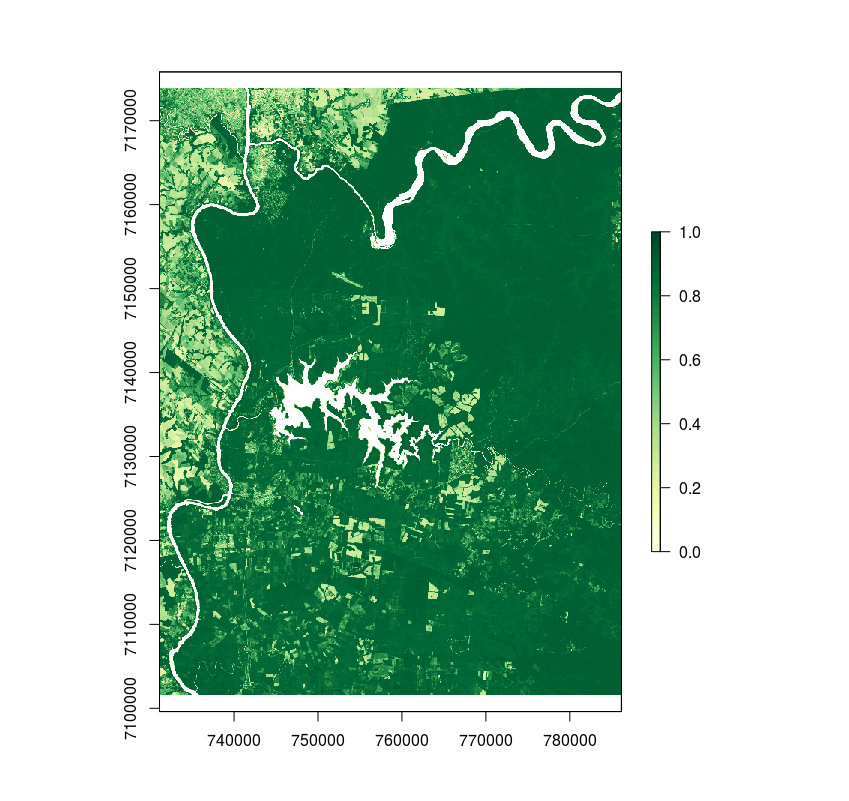
\includegraphics[scale=0.6]{ndvi_fig.png}
    \end{center}
    \caption{Mapa del NDVI en escala de verdes.}
    \label{fig:ndvifig}
    \end{figure}

\end{exa}

El paquete \texttt{RStoolbox} tiene varias herramientas que nos ayudan a
calcular los \'indices espectrales. Veamos por ejemplo como calcular el NDVI y el
EVI.

\begin{exa}
    Para calcular los \'indices mediante la funci\'on \texttt{spectralIndices} debemos
    especificar con que raster trabajamos y que bandas corresponden a cada
    longitud de onda
    \begin{lstlisting}
    indices.2016 <- spectralIndices(ref.2016,
                                    blue="blue", red="red", nir="nir",
                                    indices=c("NDVI","EVI"))
    plot(indices.2016,col=cols, zlim=c(0,1))
    \end{lstlisting}
    En este caso, vemos que la funci\'on \texttt{espectralIndices} necesita al
    menos 3 par\'ametros
    \begin{itemize}
        \item Una imagen.
        \item A que zona del espectro corresponde cada banda.
        \item Los \'indices que queremos calcular
    \end{itemize}
     \begin{figure}[h!]
     \begin{center}
         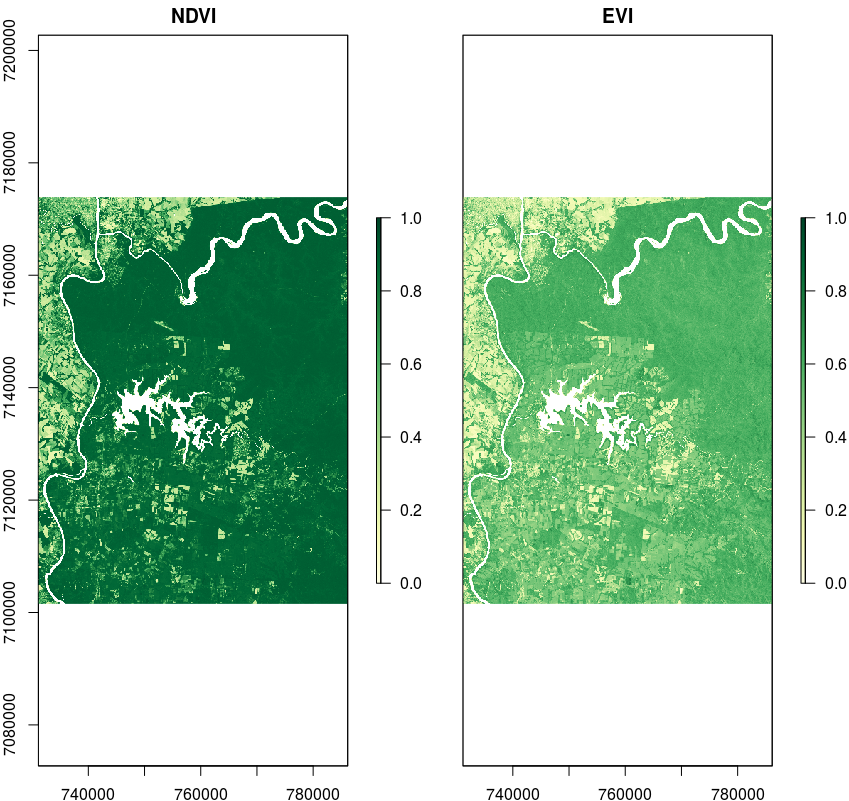
\includegraphics[scale=0.6]{evi-ndvi.png}
     \end{center}
     \caption{Graficos del EVI y el NDVI para la imagen seleccionada.}
     \label{fig:evi-ndvi}
     \end{figure}

\end{exa}

\begin{act}
    Calcule el NDVI y el EVI para el año 2000 utilizando la imagen landsat 7.
\end{act}

\begin{act}
    Calcule y grafique todos los \'indices posibles que involucren a las bandas
    roja e infrarrojo cercano de Landsat 8. Puede ayudarse con el comando
    \texttt{?spectralIndices}.
\end{act}

\section{C\'alculo de la l\'inea de suelo}

La l\'inea de suelo es una cantidad que definimos en teledetecci\'on que aporta
informaci\'on sobre las imagen que estamos analizando y sirve para incorporar
los efectos de la reflectancia del suelo en el c\'alculo de \'indices.
Veamos como hacerlo con la libreria \texttt{landsat}

\begin{exa}
    Calculemos la l\'inea de suelo a partir de la imagen Landsat 8.
    Para esto necesitamos enmascarar las zonas con
    cobertura de agua y nubes.
    \begin{lstlisting}
    mask.2016 <- raster("raster_data/LC82240782016304/LC82240782016304LGN00_cfmask.tif")
    masked.2016 <- mask(ref.2016, mask=mask.2016, inverse=TRUE,
                        maskvalue=0, updatevalue=255)
    masked.2016[masked.2016<=0] <- 255
    \end{lstlisting}
    de esta forma enmascaramos todos los valores con nubes, agua y donde la
    reflectancia obtenida es cero con el valor 255.
    Calculamos ahora la l\'inea de suelo y la mostramos en un scatterplot
    \begin{lstlisting}
    bsl.2016 <- BSL(as.matrix(masked.2016$red), as.matrix(masked.2016$nir),
                    method="quantile")
    plot(ref.2016$red, ref.2016$nir)
    abline(bsl.2016$BSL,col="red")
    \end{lstlisting}
    Obtenemos como resultado el gr\'afico de (Figura \ref{fig:soil}). Podemos consultar
    los demas par\'ametros imprimiendo la variable \texttt{bsl.2016}.
    \begin{figure}[h!]
    \begin{center}
        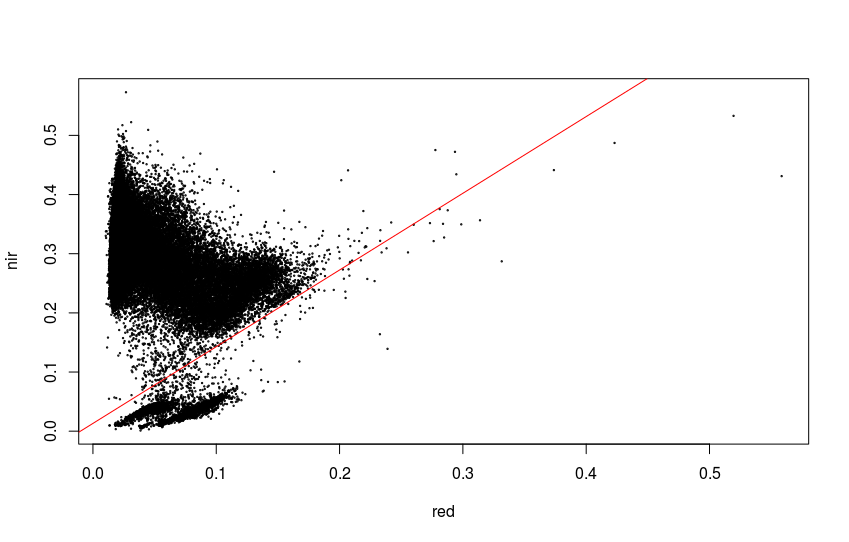
\includegraphics[scale=0.6]{soil.png}
    \end{center}
    \caption{L\'inea de suelo sobre el scatterplot nir-red}
    \label{fig:soil}
    \end{figure}

\end{exa}

\begin{act}
    Calcule el tSAVI utilizando la l\'inea de suelo.
\end{act}

\begin{act}
    Calcule la l\'inea de suelo sin enmascarar la imagen y dibuje el
    scatterplot conto con ella.
\end{act}

\begin{act}
    Obtenga la l\'inea de suelo y calcule el \'indice tSAVI para la imagen del año
    2000.
\end{act}

\section{Estimaci\'on de par\'ametros biof\'isicos}

Finalmente, veamos como se puede obtener datos biof\'isicos a partir de los
\'indices de vegetaci\'on para realizar mapas de
porcentaje de cobertura, productividad, etc.

\begin{exa}
    Comenzamos calculando el NDVI para el año 2016, y utilizando la capa
    muestreo, hacemos una extracci\'on estadi\'stica sobre la misma.
    \begin{lstlisting}
    vector <- readOGR(dsn="vector_data/", layer="muestreo")
    datos <- extract(ndvi.2016,vector)
    DF <- data.frame(vector@data,datos)
    pairs(DF)
    \end{lstlisting}

    Obtendremos un gr\'afico que presenta los scatterplots entre las bandas, su
    correlaci\'on e histogramas.
    Vemos que la superficie cubierta por vegetaci\'on var\'ia
    linealmente con el NDVI\@. Por lo tanto, los utilizaremos para hacer un ajuste de nuestro modelo

    \begin{lstlisting}
    lm.2016 <- lm(fcover~ndvi, data=muestreo)
    plot(muestreo$ndvi, mustreo$fcover)
    abline(lm.2016, col="red")
    summary(lm.2016)
    \end{lstlisting}

    de esta forma obtenemos los par\'ametros de nuestro ajuste.

    Para aplicar el modelo a nuestro raster hacemos
    \begin{lstlisting}
    fcover.2016 <- predict(ndvi.2016,lm.2016)
    plot(fcover.2016)
    \end{lstlisting}
\end{exa}

\begin{act}
    Genere los modelos de lai, fapar y fcover para el año 2016 y
    realice mapas de dichas variables.
\end{act}

\begin{act}
    Utilizando los modelos obtenidos para 2016 realice
    los mapas de lai, fapar y fcover del año 2000. ¿Que suposici\'on est\'a
    haciendo? Compare distintas zonas de los modelos en el qgis.
\end{act}


\chapter{Geometr\'ia espectral}
\label{rotaciones}
En nuestra cuarta pr\'actica trabajemos con rotaciones en el espacio espectral.
Apuntamos a poder incorporar conceptos como dimensionalidad y
correlaci\'on entre bandas, que nos ayuden a utilizar mejor la informaci\'on
satelital.

Son nuestros objetivos:

\begin{itemize}
    \item Aplicar la transformada tasseled cap a una imagen multiespectral e
        interpretar el significado de cada banda.
    \item Aplicar la transformada por componentes principales a una imagen
        multiespectral e interpretar el resultado.
    \item Aplicar la transformada por componentes principales a un stack
        de bandas multiespectrales de distintas fechas e interpretar los resultados.
    \item Extraer informaci\'on de series temporales de \'indices espectrales.
\end{itemize}

\section{C\'alculo de la transformada tasseled cap para una imagen landsat}

Comencemos calculando la transformada tasseled cap para una imagen Landsat 8. \'Esta
ser\'a la primer rotaci\'on que utilizaremos en el curso cuya la
interpretaci\'on es bastante sencilla. Usaremos el paquete
\texttt{RStoolbox}.

\begin{exa}
    Para cualcular la transformada por componentes principales comenzamos
    abriendo la imagen Landsat 8 desde el metadado y convirti\'endola a reflectancia
    a tope de la cobertura, como vimos en las clases anteriores.
    \begin{lstlisting}
    xml.2016 <- readMeta("raster_data/LC82240782016304/LC82240782016304LGN00.xml")
    ref.2016 <- stackMeta(xml.2016, quantity = "sre")
    scaleF <- getMeta(ref.2016,xml.2016, what = "SCALE_FACTOR")
    ref.2016 <- ref.2016 * scaleF
    ref.2016 <- ref.2016[[-1,]]
    names(ref.2016) <- c("blue","green","red","nir","swir1","swir2")
    \end{lstlisting}

    Analizamos ahora el espacio rojo-infrarrojo cercano y rojo-verde para la imagen

    \begin{lstlisting}
    B1 <- xyplot(nir~red,data=ref.2016)
    B2 <- xyplot(red~green,data=ref.2016)
    print(B1,split=c(1,1,2,1),more=TRUE)
    print(B2,split=c(2,1,2,1),more=FALSE)
    \end{lstlisting}

    obteniendo como scatterplots (Figura \ref{fig:green-red}).

    \begin{figure}[h!]
    \begin{center}
        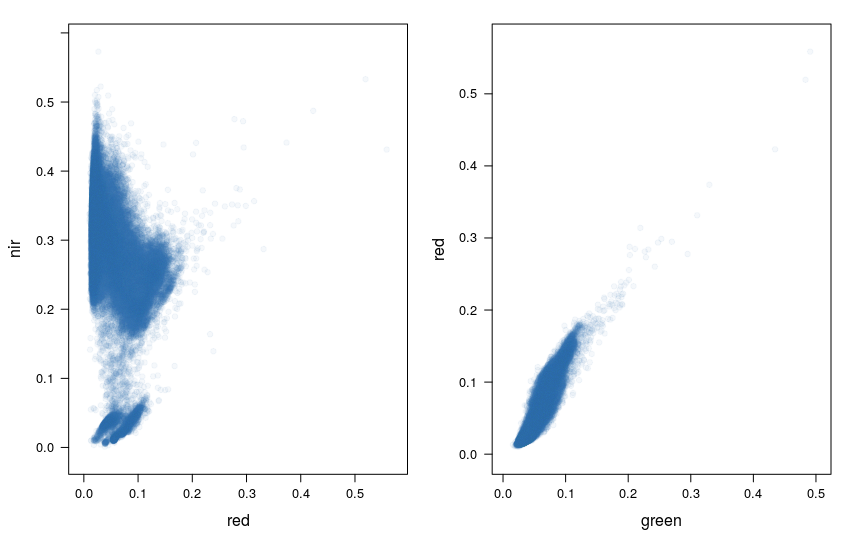
\includegraphics[scale=0.6]{red-nir-green.png}
    \end{center}
    \caption{Scatterplot verde-rojo y nir-red.}
    \label{fig:green-red}
    \end{figure}

    Calculemos ahora la transformada tasseled cap. Para eso usamos la funci\'on
    \texttt{tasseledCap} del paquete \texttt{RStoolbox}.
    \begin{lstlisting}
    tsc.2016 <- tasseledCap(ref.2016,sat="Landsat8OLI")
    \end{lstlisting}
    Tendremos una imagen de tres bandas, \emph{brillo}, \emph{verdor} y
    \emph{humedad}. Podemos graficar cada una de las bandas por separado con el
    comando \texttt{plot(tsc.2016)} o todas juntas con \texttt{plotRGB(tsc.2016,r=1,g=2,b=3, stretch="lin")}
\end{exa}

\begin{act}
    Calcule la transformada tasseled cap para la imagen Landsat 7 del año 2000.
\end{act}

\section{C\'alculo de la transformada por componentes principales}

Veamos ahora como calcular la transformada por componentes principales. Utilizaremos la
herramienta \texttt{rasterPCA} del paquete \texttt{RStoolbox}.

\begin{exa}
    Comencemos analizando la transformada por componentes principales de la
    imagen de 2016. Miremos primero los scatterplots con el comando \texttt{pairs(ref.2016)}
    obteniendolos (Figura \ref{fig:pairs2})
    \begin{figure}[h!]
    \begin{center}
        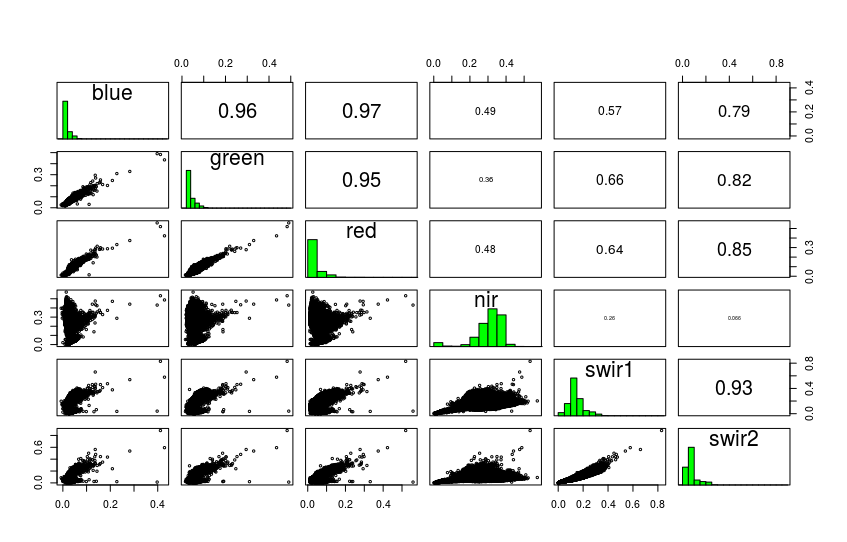
\includegraphics[scale=0.4]{pairs.png}
    \end{center}
    \caption{Scaterplots y coeficientes de correlaci\'on para la imagen Landsat 8.}
    \label{fig:pairs2}
    \end{figure}

    Mirando el resumen de la imagen vemos que hay varias bandas muy
    correlacionadas entre s\'i, como las del visible, mientras que otras lo
    estan poco, como el infrarrojo cercano y el infrarrojo de onda corta. Por lo tanto, esperamos que no
    todas las bandas sean necesarias para explicar el comportamiento de la
    imagen, al menos en el nivel de detalle m\'as bajo.

    Apliquemos entonces la transformada por componentes principales y veamos que
    sucede

    \begin{lstlisting}
        pca.2016 <- rasterPCA(ref.2016)
        summary(pca.2016$model)
    \end{lstlisting}

    El sumario del modelo obtenidos,
    \begin{Verbatim}[fontsize=\small]
    Importance of components:
                               Comp.1     Comp.2     Comp.3      Comp.4 ...
    Standard deviation     0.08079854 0.07808556 0.01242745 0.006488765 ...
    Proportion of Variance 0.50850204 0.47492732 0.01202957 0.003279516 ...
    Cumulative Proportion  0.50850204 0.98342936 0.99545892 0.998738441 ...
    \end{Verbatim}

    Al observar las varianzas, vemos que las 3 primeras explican m\'as que el
    99.5\% de la variabilidad de la imagen. Es decir que, de las 6 bandas de
    Landsat 8 en esta imagen, 3 nos alcanza para explicar casi todo el
    comportamiento. Analisemos la primera, usando el comando
    \texttt{loadings(pca.2016\$model)} para ver como son las componentes.

    \begin{Verbatim}[fontsize=\small]
    oadings:
          Comp.1  ...
    blue
    green
    red   -0.128  ...
    nir   -0.575  ...
    swir1 -0.663  ...
    swir2 -0.451  ...
    \end{Verbatim}

    La primer componente pesa siempre con el mismo signo, a
    todas las bandas. Podemos interpretarla como un
    brillo negativo y esperar que sea m\'as alta cuando miramos zonas de la imagen que
    tengan menos reflectancia en promedio. La segunda componente, presenta diferencia
    entre los valores del infrarrojo cercano y el resto de la bandas. Esta ser\'a alta
    en presencia de vegetaci\'on y baja en su ausencia. La componente tres se comporta
    de forma similar pero con las bandas del infrarrojo medio, por lo tanto podemos
    interpretarla como una componente que varia seg\'un el contenido de humedad.
\end{exa}

\begin{act}
    Calcule y analice la transformada por PCA de la imagen Landsat 7 del año
    2000.
\end{act}

\section{Algunas ideas sobre series temporales}

Empecemos esta seccion con una actividad

\begin{act}
    Aplique la transformada por componentes principales al stack de bandas del
    año 2000 y 2016.
\end{act}

Veamos que pasa al trabajar con series temporales de \'indices.

\begin{exa}
    Otra aplicaci\'on de la transformada por componentes principales
    es el an\'alisis de series temporales.
    \begin{lstlisting}
    ndvi.list <- list.files("raster_data/MOD13Q1/NDVI/", pattern = "*.tif$",
                             full.names = TRUE)
    ndvi.stack <- stack(ndvi.list)
    \end{lstlisting}
    una vez abierta la imagen la convertimos a valores entre -1 y 1 e
    interpolamos los valores faltantes.
    \begin{lstlisting}
    ndvi.stack <- ndvi.stack/1e4
    ndvi.stack <- approxNA(ndvi.stack)
    writeRaster(ndvi.stack,"ndvi-series.tif")
    \end{lstlisting}
    Una vez interpoladas las fechas donde no hab\'ia datos de NDVI, podemos
    abrirla en el QGIS y analizar distintas zonas de la imagen.

    Utilizando la herramienta de identificar objetos espaciales podemos
    consultar como es el comportamiento de la serie temporal para cada p\'ixel.

    \begin{figure}[h!]
    \begin{center}
        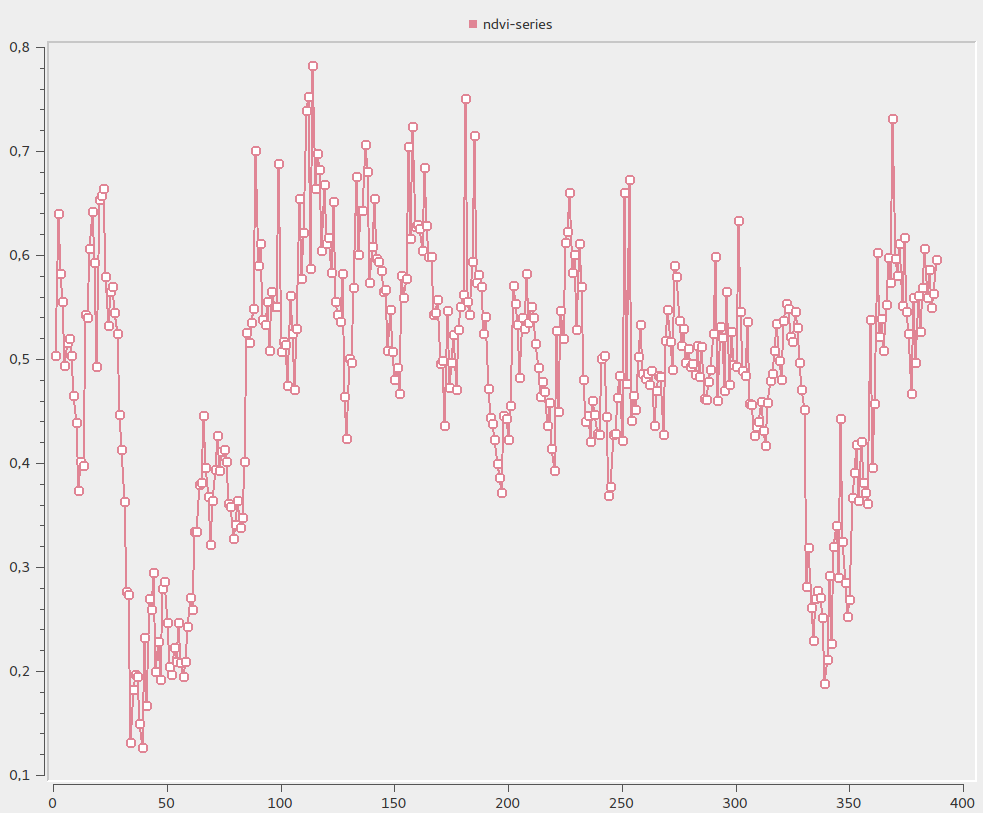
\includegraphics[scale=0.3]{series.png}
    \end{center}
    \caption{Serie temporal de valores de NDVI.}
    \label{fig:series}
    \end{figure}

    Vemos que distintas zonas tienen distintos comportamientos intra e
    interanual.

    Podemos analizar el promedio y el desv\'io standar para cada p\'ixel de la
    imagen
    \begin{lstlisting}
    ndvi.mean <- mean(ndvi.stack)
    plot(ndvi.mean)
    ndvi.sd <- calc(ndvi.stack, fun=sd)
    plot(ndvi.sd)
    \end{lstlisting}
\end{exa}


\begin{act}
    Grafique las primeras 4 componentes de la transformada por componentes
    princiales de la imagen del stack de NDVI\@. ¿Qu\'e zonas puede identificar en la
    primera? ¿Qu\'e zonas se distinguen en la segunda? ¿Qu\'e comportamiento encuentra
    en la tercera y cuarta?
\end{act}


\part{Variables discretas}

\chapter{Clasificacion no supervisada de imagenes}
\label{otrolado}
En la quinta clase del curso, trabajaremos con clasificaci\'on no supervisada
de im\'agenes satelitales. Son nuestros objetivos:

\begin{itemize}
  \item Usar la herramienta de clasificaci\'on no supervisada.
  \item Aprender a indentificar clases espectrales en catego\'ias de uso y cobertura.
  \item Incorporar informaci\'on no espectral a las clasificaciones como
  pueden ser datos temporales o informaci\'on espacial.
  \item Aplicar la transformada por componentes principales para reducir la dimensionalidad
  y seleccionar los datos mas relevantes previos a las clasificaciones.
\end{itemize}

\section{Clasificaci\'on mediante el m\'etodo k-means}

Cargaremos primero la imagen landsat 8 y habilitaremos la opcion para escribir
el header de ENVI\@.

\begin{lstlisting}
    rasterOptions(addheader = "ENVI")
    xml.2016 <- readMeta("raster_data/LC82240782016304/LC82240782016304LGN00.xml")
    ref.2016 <- stackMeta(xml.2016, quantity = "sre")
    scaleF <- getMeta(ref.2016,xml.2016, what = "SCALE_FACTOR")
    ref.2016 <- ref.2016 * scaleF
    ref.2016 <- ref.2016[[-1,]]
    names(ref.2016) <- c("blue","green","red","nir","swir1","swir2")
\end{lstlisting}

Veamos como clasificar una imagen usando el m\'etodo k-means en R. Vamos a usar
los paquetes \texttt{raster} y \texttt{RStoolbox}

\begin{exa}
    Comenzamos seteando la semilla para el geneador de n\'umeros aleatorios con el
    comando \texttt{set.seed(42)}. De esta forma la serie de n\'umeros aleatorios
    es la misma para todos.

    Luego clasificamos la imagen y la guardamos como vimos en las clases anteriores.
    \begin{lstlisting}
    set.seed(42)
    kmeans.2016 <- unsuperClass(ref.2016, nClasses = 5, nStarts = 100,
                                nSamples = 100)
    writeRaster(kmeans.2016$map, "raster_data/processed/kmeans2016",
                datatype="INT1U")
    \end{lstlisting}

    En este caso estamos solamente usando 5 clases espectrales. Podemos ahora graficar por separado cada una de las clases
    \begin{lstlisting}
        clases.2016 <- layerize(kmeans.2016$map)
        plot(clases.2016)
    \end{lstlisting}
    \begin{figure}
      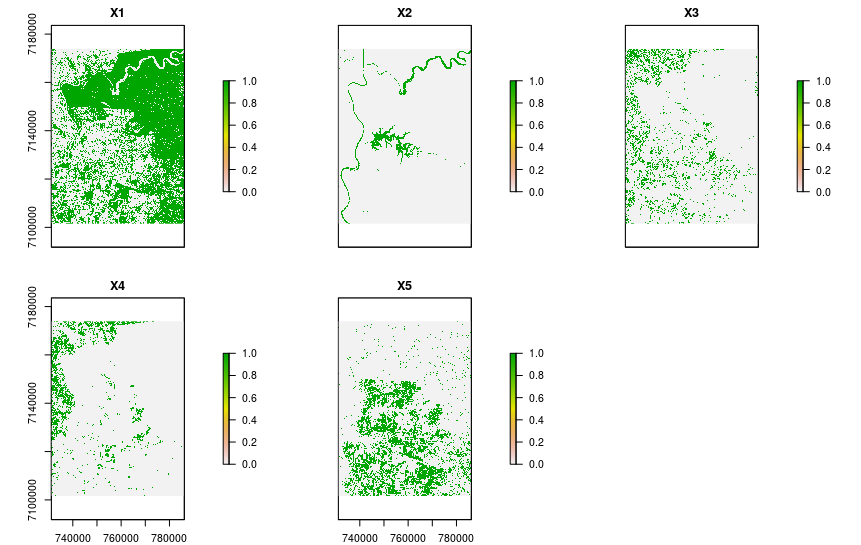
\includegraphics{clases_5.png}
      \caption{Clases generadas por el algoritmo kmeans para 5 clases.}
      \label{fig:clases5}
    \end{figure}
    Abriremos la imagen ahora en el qgis e identificaremos cada una de las clases realiando interpretacion visual de la imagen.

    Para realizar la identificacion primero vamos al menu \menu{propiedades de la
    imagen, Estilo, Tipo de renderizacion, Unibanda pseudocolor}. Elegimos de modo
    Intervalo Igual y en numero de clases ponemos con el minimo en 1 y el maximo en
    5. En estilo de color elegimos colores aleatorios. Iremos luego cambiando los
    colores uno a uno por un color brillante e identificado a que cobertura
    pertenece dicha clase espectral.

    Construiremos con ella una tabla como la siguiente

    \begin{verbatim}
        id  class
        1   2
        2   7
        3   1
        4   1
        5   1
    \end{verbatim}

  que guardaremos en un archivo de texto con el nombre \file{class}. El mismo lo utilizaremos para realizar
  la fusion de clases.

  Una vez conocidas las categorias de uso y cobertura correspondientes a cada
  clase espectral podemos combinarlas

  \begin{lstlisting}
      clases.2016 <- read.delim("aux_data/class.txt")
      reclas.2016 <- subs(kmeans.2016$map, clases.2016)
  \end{lstlisting}

  para graficar ahora con los colores prestablecidos definimos la paleta de colores y fijamos los limites

  \begin{lstlisting}
    colores = c('#b2df8a','#33a02c',
                '#fdbf6f','#ff7f00',
                '#fb9a99','#e31a1c',
                '#a6cee3','#1f78b4')
    plot(reclas.2016, col=colores, zlim=c(1,8))
  \end{lstlisting}
  \begin{figure}
    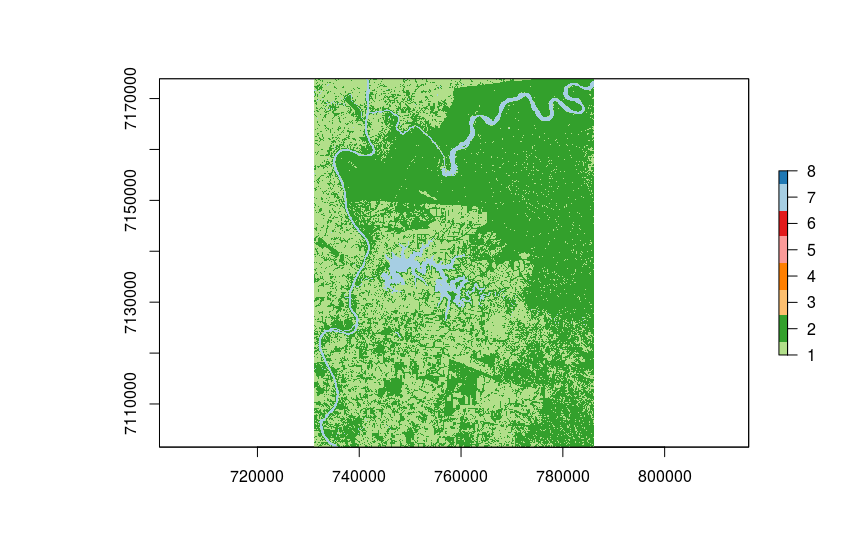
\includegraphics{kmeans-colores.png}
    \caption{Imagen clasificada por el metodo kmeans con 5 clases.}
    \label{fig:kmean5}
  \end{figure}
\end{exa}

\begin{exa}
  Hagamos un analisis espectral de las imagenes clasificadas antes y despues de la fusion.
  Para esto utilizaremos a la imagen clasificada como mascara para asignar los colores
  al scatterplot. Para esto usaremos la libreria \texttt{rasterVis}.

  Agregamos la imagen clasificada a las bandas de la imagen en reflectancia y luego
  hacemos los scatterplot segun la clase espectral o de informacion como

  \begin{lstlisting}
    stack.2016 <- stack(ref.2016, reclas.2016)
    xyplot(nir+swir1~red, groups=MC_ID, data=stack.2016)
  \end{lstlisting}
  Vemos que las clases espectrales pueden unirse en clases de informacion y que algunas clases de informacion no se separan en distintas clases espectrales (figuras \ref{fig:esk}).
  \begin{figure}
    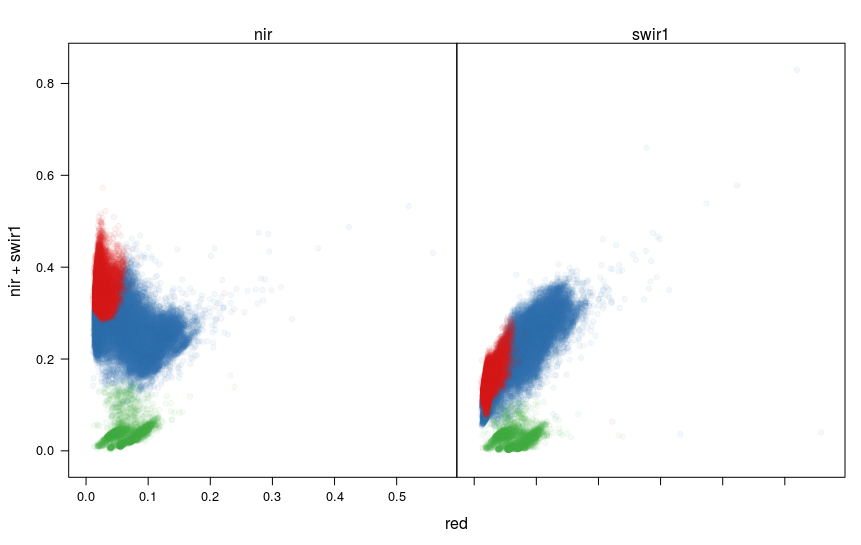
\includegraphics{kmeans-es.png}
    \caption{Espacio espectral clasificado por kmeans.}
    \label{fig:esk}
  \end{figure}

\end{exa}

\begin{exa}
  Repitamos este analisis pero con 100 clases espectrales. El algoritmo es el mismo
  pero ahora vamos a usar el parametro nClasses igual a 100.
  \begin{lstlisting}
  set.seed(42)
  kmeans.2016b <- unsuperClass(ref.2016, nClasses = 100, nStarts = 100,
                              nSamples = 1000)
  writeRaster(kmeans.2016b$map, "raster_data/processed/kmeans2016b",
              datatype="INT1U", overwrite=TRUE)
  clasesb.2016 <- read.delim("aux_data/class100.txt")
  reclasb.2016 <- subs(kmeans.2016b$map, clasesb.2016)
  plot(reclasb.2016, col=colores, zlim=c(1,8))
  \end{lstlisting}

  \begin{figure}
    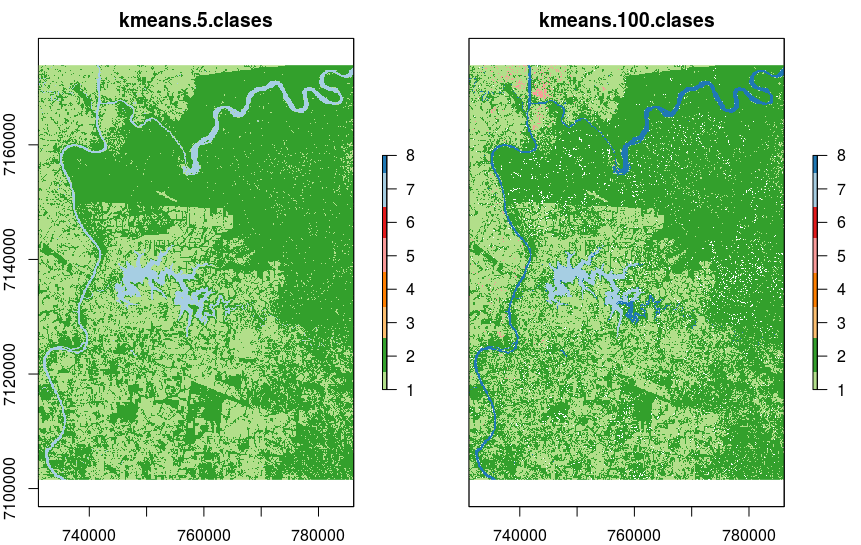
\includegraphics{5v100.png}
    \caption{Comparacion entre la clasificacion con 5 clases y 100 clases espectrales.}
    \label{fig:5v100}
  \end{figure}

  Comparamos nuevamente los espacios de fase entre la clasificacion obtenida a partir de 5 y 100 clases espectrales
  \begin{lstlisting}
    stackb.2016 <- stack(ref.2016, reclasb.2016)
    xyplot(nir+swir1~red, groups=MC_ID, data=stack.2016)
    xyplot(nir+swir1~red, groups=MC_ID, data=stackb.2016)
  \end{lstlisting}

  Vemos en este caso que somos capaces de separar todas las clases de informacion en el espacio de fases.

\end{exa}

\begin{act}
    Vuelva a repetir la clasificacion utilizando la imagen obtenida de la transformada por componentes principales descartando las bandas que aporten menos informacion.
\end{act}

\begin{act}
  Repita la clasificacion para la imagen landsat 7 del año 2000.
\end{act}


\section{Informacion espacio-temporal}
Con el fin de mejorar la clasificacion podemos incorporar informacion espacial y temporal a la informacion radiometrica. De esta forma estaremos, al momento de clasificar los pixeles, ya no trabajando en un espacio espectral si no en uno mas amplio. Veamos como hacer esto.

\begin{exa}
  Para incorporar informacion espacial sobre el contexto del p\'ixel, podemos
  hacerlo tanto antes como despu\'es de la clasificaci\'on. Nos centraremos
  en este caso en como hacerlo antes.

  Calculamos primero la variabilidad local de brillo para la banda pancromatica
  de la imagen Landsat 8 como

  \begin{lstlisting}
    pan.2016 <- raster("raster_data/LC82240782016304LGN00/LC82240782016304LGN00_B8.TIF")
    window <- matrix(1,nrow=5, ncol=5)
    sd.2016<-focal(pan.2016,w=window,fun=sd)
    plot(log(sd.2016,base = 10), zlim=c(1,4))
  \end{lstlisting}

  Vemos que las zonas con mayor presencia de urbanizaciones presentan una mayor variabilidad que aquellas con menor presencia.

  \begin{figure}
    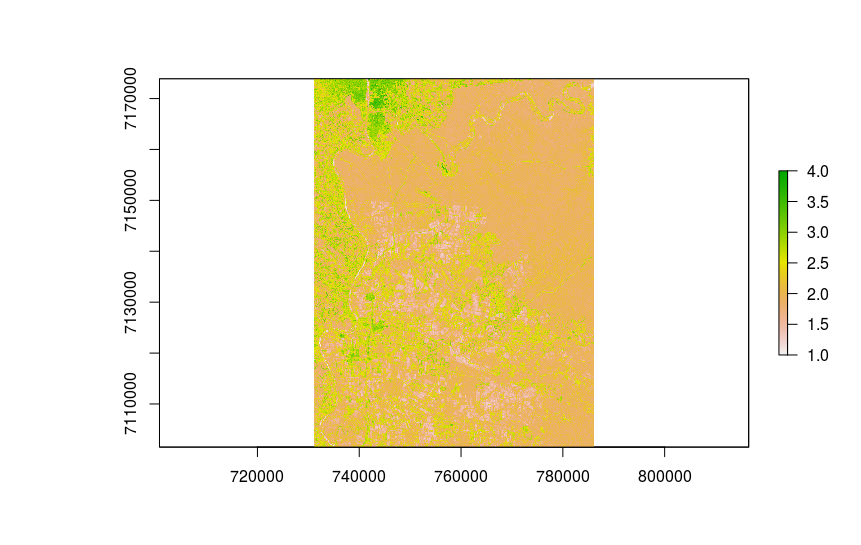
\includegraphics{pan-sd.png}
    \caption{Desvio standar para una ventana de 5 pixeles por 5 pixeles en escala logaritmica.}
    \label{fig:pansd}
  \end{figure}

  Una vez obtenida la banda de desvio standar, podemos agregarla a las demas, luego
  de remuestrearla haciendo

  \begin{lstlisting}
    sd.2016 <- aggregate(sd.2016, fact=2, fun=mean)
    stack(ref.2016, sd.2016)
    pca.2016 <- rasterPCA(stack(ref.2016, sd.2016), spca = TRUE)
  \end{lstlisting}

  \begin{Verbatim}[fontsize=\small]
  Importance of components:
                            Comp.1    Comp.2    Comp.3     Comp.4      Comp.5      Comp.6      Comp.7
  Standard deviation     2.1592402 1.1821570 0.8392878 0.40888073 0.196591748 0.143753334 0.096362617
  Proportion of Variance 0.6660455 0.1996422 0.1006292 0.02388335 0.005521188 0.002952146 0.001326536
  Cumulative Proportion  0.6660455 0.8656876 0.9663168 0.99020013 0.995721318 0.998673464 1.000000000
  \end{Verbatim}

  Vemos en este caso, analizando el sumario, que la banda de textura agrega informacion
  con respecto a la solo disponible al utilizar las bandas en radiancia.
\end{exa}

\begin{act}
  Repita el ejemplo para la imagen landsat 7 del año 2000. Clasifique por el metodo de kmeans las imagenes de los años 2000 y 2016.
\end{act}

\begin{exa}
  Para incorporar informacion del contexto temporal, agregaremos a la informacion
  espectral informacion sobre la variacion del indice de vegetacion durante el
  año en que se tomo la imagen. Primero cargamos las imagenes modis del 2016

  \begin{lstlisting}
    list.2016 <- list.files("raster_data/MOD13Q1/NDVI/", pattern = "MOD13Q1.A2016+.*tif", full.names = TRUE)
    ndvi.2016 <- stack(list.2016)/1e4
    ndvi.2016 <- approxNA(ndvi.2016)
    sd.2016 <- calc(ndvi.2016, fun = sd)
    me.2016 <- calc(ndvi.2016, fun = mean)
    plot(stack(me.2016,sd.2016))
  \end{lstlisting}

  Una vez hecho esto, resampleamos el promedio y el desvio de la serie temporal
  y lo unimos a las imagenes en reflectancia, sobre las cuales calcularemos
  la transformada por componentes principales.

  \begin{lstlisting}
    sd.2016 <- resample(sd.2016, ref.2016, method="ngb")
    me.2016 <- resample(me.2016, ref.2016, method="ngb")
    pca.2016 <- rasterPCA(stack(ref.2016, me.2016, sd.2016), spca = TRUE)
    summary(pca.2016$model)
  \end{lstlisting}

  podemos ahora seleccionar las 4 componentes que explican el 99\% de comportamiento de la imagen y clasificarla.

  \begin{Verbatim}[fontsize=\small]
    Importance of components:
                              Comp.1    Comp.2     Comp.3     Comp.4     Comp.5      Comp.6      Comp.7      Comp.8
    Standard deviation     2.3109360 1.3111953 0.69083373 0.48042475 0.41555630 0.176127381 0.139538990 0.095410787
    Proportion of Variance 0.6675532 0.2149042 0.05965641 0.02885099 0.02158588 0.003877607 0.002433891 0.001137902
    Cumulative Proportion  0.6675532 0.8824573 0.94211373 0.97096472 0.99255060 0.996428206 0.998862098 1.000000000
  \end{Verbatim}
\end{exa}

\begin{act}
  Repita el ejemplo para la imagen Landsat 7 del año 2000. Clasifique por el metodo de kmeans las imagenes de los años 2000 y 2016.
\end{act}


\chapter{Clasificacion supervisada de imagenes}
\label{educando}
En la sexta clase del curso, continuamos trabajando con algor\'itmos de clasificaci\'on de im\'agenes, centrandonoces ne este caso en los no supervisados. Son nuestros objetivos:

\begin{itemize}
  \item Poder realizar clasificaciones no supervisadas utilizando los distintos algoritmos que se encuentran en R.
  \item Calcular la distancia espectral entre como forma de determinar la separabilidad de dos clases espectrales.
  \item Comparar utilizando la entropia de un pixel que coberturas presentan  mayor confusion al momento de la clasificacion.
\end{itemize}

Cargaremos primero la imagen landsat 8 y habilitaremos la opcion para escribir el header de ENVI\@. Usaremos en primer lugar los paquetes \texttt{raster}, \texttt{rgdal}, \texttt{RStoolbox} y \texttt{rasterVis}. Ademass para las clasificaciones vamos a usar las librerias \texttt{e1071}

\begin{lstlisting}
    rasterOptions(addheader = "ENVI")
    xml.2016 <- readMeta("raster_data/LC82240782016304/LC82240782016304LGN00.xml")
    ref.2016 <- stackMeta(xml.2016, quantity = "sre")
    scaleF <- getMeta(ref.2016,xml.2016, what = "SCALE_FACTOR")
    ref.2016 <- ref.2016 * scaleF
    ref.2016 <- ref.2016[[-1,]]
    names(ref.2016) <- c("blue","green","red","nir","swir1","swir2")
    vector <- readOGR(dsn="vector_data", layer="entrenamiento")
\end{lstlisting}

\section{Clasificador por m\'axima verosimilitud}

Empecemos con la clasificacion por el metodo de maxima verosimilitud, para esto necesitamos del paquete

\begin{lstlisting}
    colores = c('#b2df8a','#33a02c',
                '#fdbf6f','#ff7f00',
                '#fb9a99','#e31a1c',
                '#a6cee3','#1f78b4')
    sup.2016 <- superClass(ref.2016, vector, responseCol = "MC_ID",
                           model = "mlc")
    plot(sup.2016$map, col=colores, zlim=c(1,8))
\end{lstlisting}

\begin{figure}[h!]
  \centering
  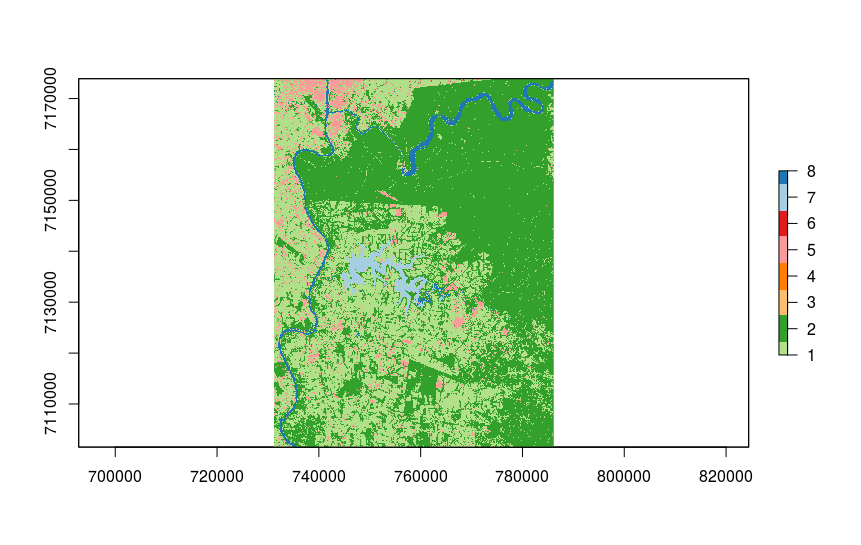
\includegraphics[width=0.7\textwidth]{mlc-MC.png}
  \caption{Clasificacion por maxima verosimilitud sin separar en clases espectrales.}
  \label{fig:MC}
\end{figure}

Cambiando el algoritmo de clasificacion en el parametro \texttt{model} podemoscalcular distintas clasificaciones supervisadas. Algunas de las vistas en clase son \texttt{mlc}, \texttt{rf} y \texttt{svmRadial}. Cada una de ellas usa alguna libreria adicional de las cargadas antes.

\begin{exa}
  Una forma de mejorar las clasificaciones supervisadas basadas en el espacio espectral es clasificar por separado distintas clases espectrales y luego unirlas en la misma clase de informacion. Veams como hacerlo.

  \begin{lstlisting}
      sup.2016b <- superClass(ref.2016, vector, responseCol = "C_ID",
                             model = "mlc")
  \end{lstlisting}

  En este caso, la columna de respuestaa es \texttt{C\_ID} y no \texttt{MC\_ID}.  Una vez realizada la clasificacion, debemos substituir los valores de cada pixel por el de la clase de informacion correspondiente. Para ello hacemos

  \begin{lstlisting}
    subs.2016 = vector@data[c(3,1)]
    sub.2016 <- reclassify(sup.2016b$map, subs.2016)
    writeRaster(sub.2016, "raster_data/processed/mlc2016",
                datatype="INT1U")
  \end{lstlisting}

    Podemos finalmente comparar las dos imagenes clasificadas lado a lado ejecuntado el comando \verb|plot(stack(sup.2016$map,sub.2016),col=colores,zlim=c(1,8))|
    \begin{figure}[h!]
      \centering
      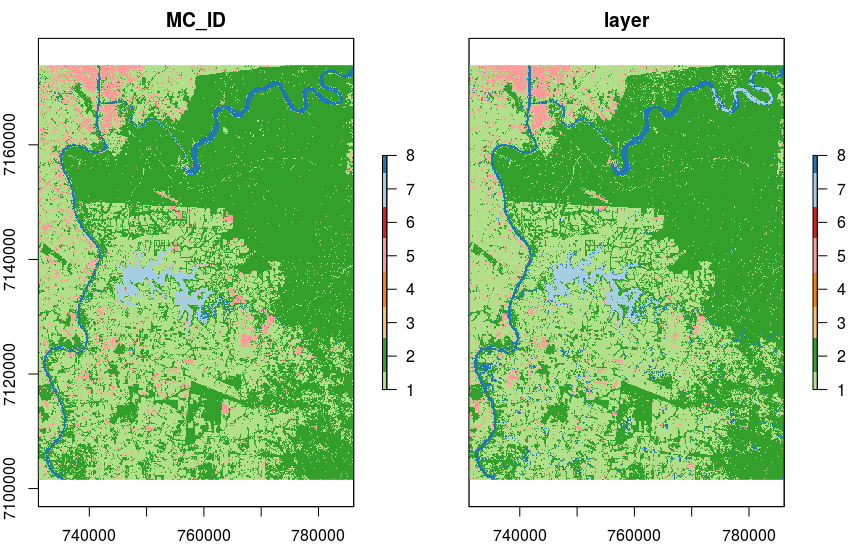
\includegraphics[width=0.7\textwidth]{mlc-comparacion.png}
      \caption{Comparacion entre la clasificacion utilizando clases de informacion y clases espectrales.}
      \label{fig:mlc}
    \end{figure}
\end{exa}

\begin{act}
    Realice clasificaciones por los distintos metodos y comparelas visualmente.
\end{act}

\begin{act}
    Agregue las bandas de textura y evolucion temporal del NDVI y vuelva a clasificar las imagenes.
\end{act}

\section{Entropia de la clasificacion}

Para poder comparar en que zonas los clasificadores presentan mas o menos dispersion podemos calcular la entropia de las distintas clasificaciones en cada pixel. Para esto utilizaremos la funcion \texttt{rasterEntropy}.

\begin{exa}
  Para esto comenzamos corriendo la clasificacion para distintos modelos, los apilados y
  despues calculamos la entropia de los mismos

  \begin{lstlisting}
      set.seed(42)
      library(e1071)
      sup.2016 <- superClass(ref.2016, vector, responseCol = "C_ID",
                           model = "mlc")
      mlc.2016 <- reclassify(sup.2016$map, subs.2016)

      library(randomForest)
      sup.2016 <- superClass(ref.2016, vector, responseCol = "C_ID",
                           model = "rf")
      rf.2016 <- reclassify(sup.2016$map, subs.2016)

      library(kernlab)
      sup.2016 <- superClass(ref.2016, vector, responseCol = "C_ID",
                           model = "svmLinear")
      svm.2016 <- reclassify(sup.2016$map, subs.2016)

      prediction_stack <- stack(mlc.2016, rf.2016, svm.2016)
      names(prediction_stack) <- c("mlc","rf","svm")
      model_entropy <- rasterEntropy(prediction_stack)
  \end{lstlisting}

  Podemos graficar la entropia de las clasificaciones como \verb|model_entropy| y ver que zonas presentan mas diferencias a la hora de la clasificacion y cuales no.
  \begin{lstlisting}
    plot(stack(prediction_stack, model_entropy),col=colores)
  \end{lstlisting}
\end{exa}
  \begin{figure}[h!]
    \centering
    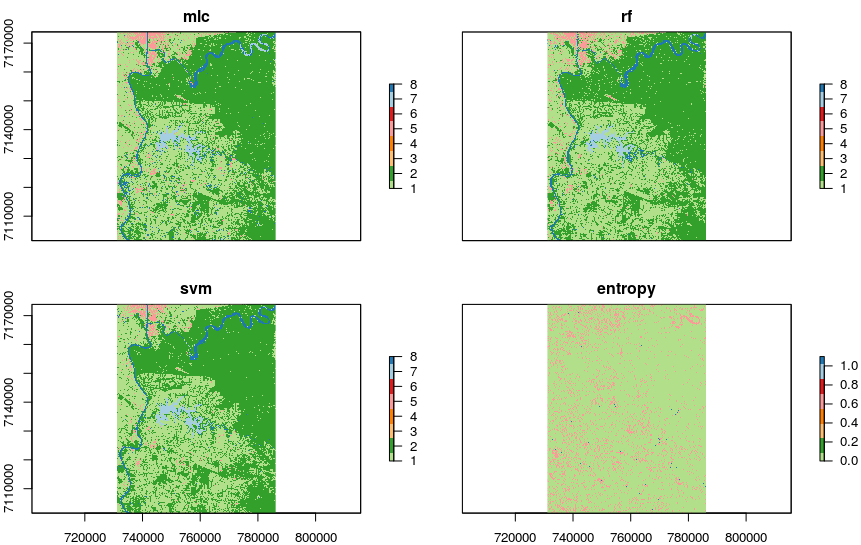
\includegraphics[width=0.7\textwidth]{comparacion-sup.png}
    \caption{Comparacion entre los distintos metodos de clasificacion supervisada usando la entropia de la clasificacion.}
    \label{fig:entropia}
  \end{figure}
\begin{act}
  Repita las clasificaciones por los metodos de arriba agregando la banda textura. Apilela junto con las clasificaciones por k-means de la clase anterior. ¿A que cobertura pertenecen las zonas con mayor variabilidad?
\end{act}


\chapter{Tecnicas pos-clasificacion}
\label{pos}
Veamos finalmente, en esta pr\'actica, algunas t\'ecnicas de posprocesamiento para im\'agenes satelitales que nos ayudaran a mejorar los valores extraidos y conocer la incerteza en su estimaci\'on. Son nuestros objetivos:

\begin{itemize}
  \item Aplicar filtros modales a las clasificaciones para eliminar p\'ixeles aislados.
  \item Calcular la presici\'on total para la clasificaci\'on y sus precisiones del usuario y productor.
  \item Estimar el error de para las superficies calculadas a partir de la imagen clasificada.
\end{itemize}

Vamos a usar los paquetes \texttt{raster}, \texttt{rgdal}, \texttt{RStoolbox} y \texttt{rasterVis}.

\section{Filtrado de clasificaciones}

Una de las primeras tareas a realizar luego de clasificar una imagen es aplicar un filtro a la misma que permite eliminar p\'ixeles aislados. Al hacerlo podremos descartar, por ejemplo, pixeles de ciudad en el medio de la selva o de selva en medio de la ciudad. Esta es otra forma de incorporar el contexto espacial a nuestras clasificaciones
\begin{exa}
  Veamos como aplicar un filtro por moda a una imagen clasificada. Comencemos cargando una imagen clasificada en R

  \begin{lstlisting}
      mlc.2016 = raster("raster_data/processed/mlc2016")
  \end{lstlisting}

  Para aplicar el filtro de 3x3 creamos una matriz con unos de 3x3 y usamos
  el comando \texttt{focal} con la funcion \texttt{modal}

  \begin{lstlisting}
    colores = c('#b2df8a','#33a02c',
                '#fdbf6f','#ff7f00',
                '#fb9a99','#e31a1c',
                '#a6cee3','#1f78b4')
    window <- matrix(1,nrow=3, ncol=3)
    mlc.3x3.2016 <-focal(mlc.2016,w=window,fun=modal)
    writeRaster(mlc.3x3.2016,"raster_data/processed/mlc3x3-2016", datatype = "INT1U", overwrite=TRUE)
    plot(mlc.3x3.2016,col=colores)
  \end{lstlisting}
  En el caso de un filtro por moda, estaremos dejando el mayor que mas veces aparezca entre los que rodean al pixel. Podemos en este caso mostrar las im\'agenes con y sin el filtro juntas (figura \ref{fig:3x3}).

  \begin{lstlisting}
    plot(stack(mlc.2016, mlc.3x3.2016),col=colores)
  \end{lstlisting}

  \begin{figure}[h!]
    \centering
    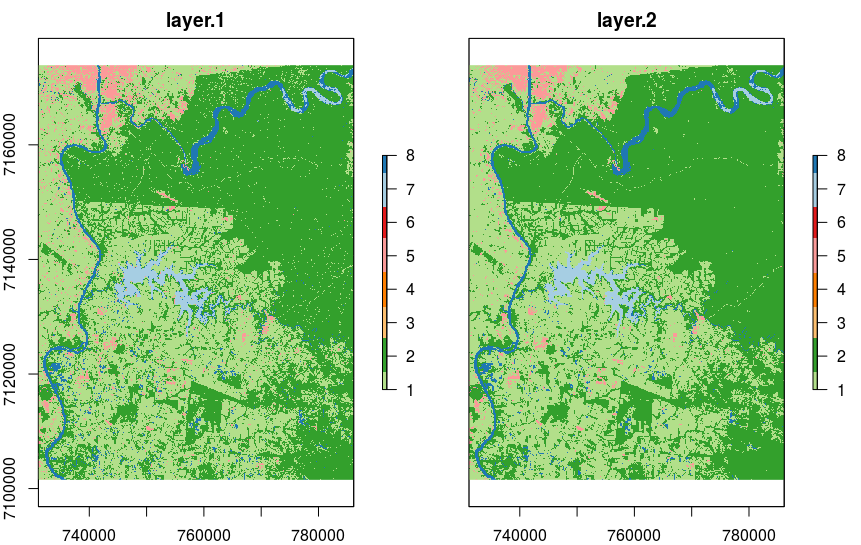
\includegraphics[scale=0.4]{filtro3x3.png}
    \caption{Imagen de la clasificacion con y sin filtro con una ventana de 3x3.}
    \label{fig:3x3}
  \end{figure}
\end{exa}

\begin{act}
    Aplique filtros de 5x5 y 7x7 para filtrar la imagen. ¿Que problemas desaparecen? ¿Que dificultad introducen?
\end{act}

\begin{act}
    Aplique el filtro de 3x3 a la imagen correspondiente al año 2000.
\end{act}

\section{Validaci\'on de clasificaciones}

El segundo procesamiento pos-clasificaci\'on, y tal vez el mas importante, es el c\'alculo de la matriz de confusi\'on para n
uestra clasificacio\'n. Haremos esto en dos partes: crearemos primero el set de datos para la validaci\'on y luego lo usaremos para calcular dicha matriz.

\begin{exa}
  Veamos como crear un set de puntos aleatorios de muestreo con QGIS. En este caso utilizaremos como unidad de muestreo al p\'ixel, pero de forma similar pueden usarse poligonos o grupos de poligonos.

  Comenzamos abriendo la imagen \file{mlc3x3-2016} en QGIS. Una vez hecho esto, vamos a vectorizar la clasificaci\'on utilizando la herramienta \menu{Raster, Conversion, Poligonizar}. Guardamos el archivo como \file{2016-3x3.shp} en la carpeta de \file{vector\_data} poniendo en nombre del campo \menu{MC\_ID} (figura \ref{fig:poligon}).

  \begin{figure}[h!]
    \centering
    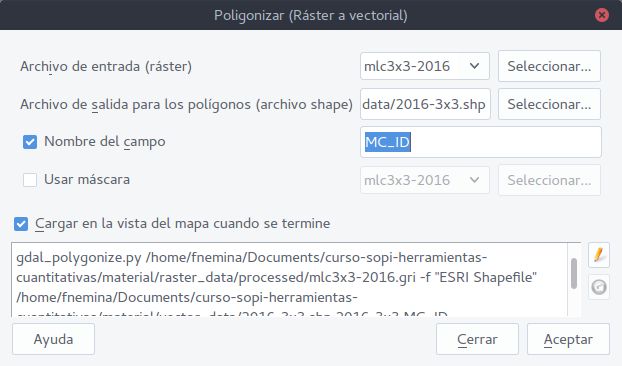
\includegraphics[scale=0.4]{poligon.png}
    \caption{Herramienta de poligonizaci\'on}
    \label{fig:poligon}
  \end{figure}

  Una vez hecho esto utilizamos la herramienta \menu{Herramientass de gesti\'on de datos, Dividir capa vectoria} y lo guardamos en la carpeta \file{vector\_data,split} (figura \ref{fig:split}).

  \begin{figure}[h!]
    \centering
    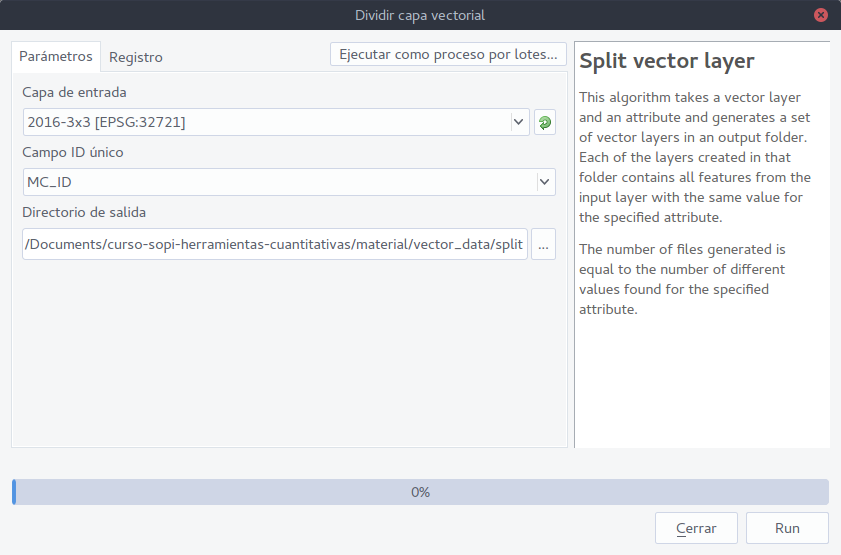
\includegraphics[scale=0.4]{split.png}
    \caption{Herramienta de divisi\'on de capa vectorial.}
    \label{fig:split}
  \end{figure}

  Cargamos luego las capas en
  QGIS, elegimos la herramienta \menu{Herramientas de investigacion, Puntos aleatorios en los limites de la capa} y hacemos click en el boton \menu{Ejecutar proceso por lotes}. Hacemos click en el boton con los tres puntos y elegimos \menu{Seleccionar del sistema de archivos}.  Seleccionamos cada capa y en numero de puntos ponemos la cantidad correspondiente a cada categoria.

  Para calcular dicha cantidad usamos el comando \texttt{freq.2016 <- freq(mlc.3x3.2016)}  para conocer las frecuencias de aparicion de cada categoria y luego con el comando  \texttt{freq.2016[,2] <- round(freq.2016[,2]/sum(freq.2016[,2])*250+50)} distribuimos  los p\'ixeles en cada categoria con 50 fijos y 50 segun la frecuencia de aparicion.
  Con una distancia minima de 100m (figura \ref{fig:dots}).

  \begin{figure}[h!]
    \centering
    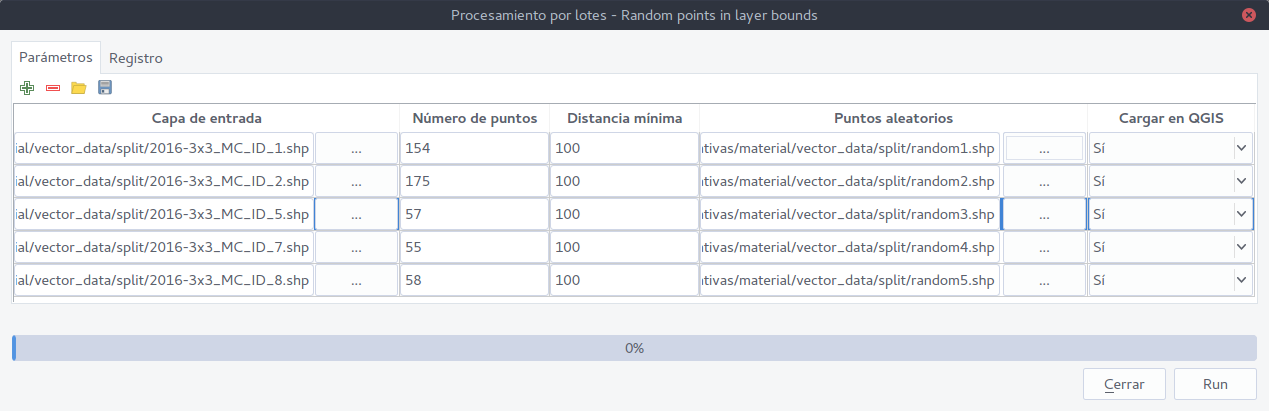
\includegraphics[scale=0.3]{random-dots.png}
    \caption{Herramienta de creaci\'on de puntos aleatorios.}
    \label{fig:dots}
  \end{figure}

  Elegimos luego en que carpeta guardar los puntos aleatorios y con que nombre y hacemos click en aceptar. Finalmente, una vez creadas las capas de puntos aleatoriosa las unimos utilizando la herramienta \menu{Herramientas de gestion de datos, Combinar capas vectoriales} con el nombre \file{val-2016.shp} (figura \ref{fig:combinar}).

  \begin{figure}[h!]
    \centering
    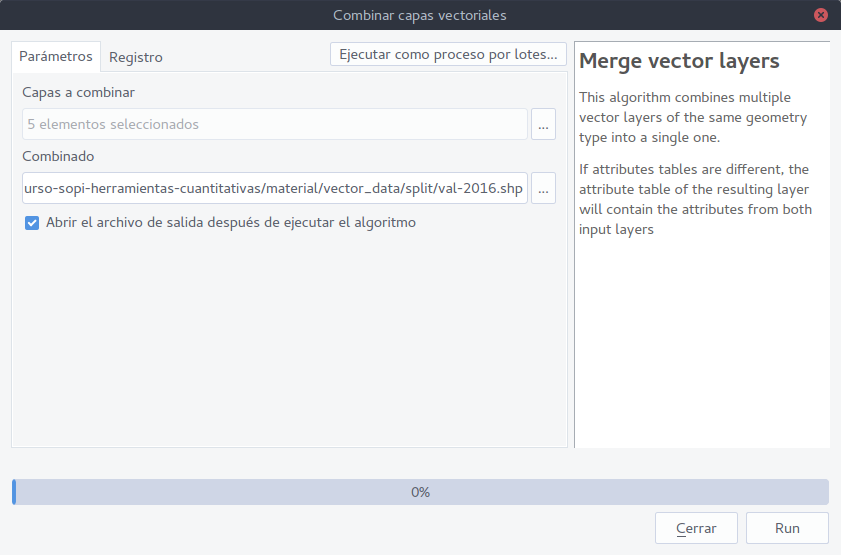
\includegraphics[scale=0.4]{combinar.png}
    \caption{Combinacion de poligonos en una capa vectorial.}
    \label{fig:combinar}
  \end{figure}

  Una vez unidas las capas editamos la tabla de atributos para agregar el campo \verb|MC_ID| y, realizando un an\'alisis visual en distintas combinaciones de bandas, asignamos a cada punto el \verb|MC_ID| de la clase de informaci\'on a la que pertenece.

  Para hacerlo podemos utilizar la misma imagen que usamos para clasificar o una de mayor resoluci\'on espacial. Una vez terminado y guardada la capa tendremos nuestra capa de validaci\'on para continuar.

\end{exa}

\begin{act}
  Construya de esta forma una serie de puntos de validaci\'on para la imagen Landsat 7 del a\~no 2000.
\end{act}

\begin{exa}

  Una vez obtenidos los puntos de validaci\'on podemos calcular la matriz de confusi\'on.  Para esto debemos cargar el pol\'igono de validaci\'on y la calculamos con la funci\'on \texttt{validateMap}.

  \begin{lstlisting}
      valid.2016 <- readOGR(dsn="vector_data", layer="validacion")
      val.2016 <- validateMap(mlc.3x3.2016,valData = valid.2016,
                                responseCol = "MC_ID")
  \end{lstlisting}

  al inspeccionar el elemento \verb|val.2016$performance| obtenemos la matriz
  de confusi\'on, la presici\'on global como \emph{Acuracy}, la presici\'on del
  productor como \emph{Sensitivity} y la del usuario como \emph{Pos Pred Value}.

  \begin{Verbatim}[fontsize=\small]
    Confusion Matrix and Statistics

              Reference
    Prediction   1   2   5   7   8
             1 150  27  14   6   2
             2   5 164   0   0   0
             5   6   0  21   0   0
             7   1   0   0  35   5
             8   3   0   0   6  54

    Overall Statistics

                   Accuracy : 0.8497
                     95% CI : (0.8153, 0.8799)
        No Information Rate : 0.3828
        P-Value [Acc > NIR] : < 2.2e-16

                      Kappa : 0.7888
     Mcnemar's Test P-Value : NA

    Statistics by Class:

                         Class: 1 Class: 2 Class: 5 Class: 7 Class: 8
    Sensitivity            0.9091   0.8586  0.60000  0.74468   0.8852
    Specificity            0.8533   0.9838  0.98707  0.98673   0.9795
    Pos Pred Value         0.7538   0.9704  0.77778  0.85366   0.8571
    Neg Pred Value         0.9500   0.9182  0.97034  0.97380   0.9839
    Prevalence             0.3307   0.3828  0.07014  0.09419   0.1222
    Detection Rate         0.3006   0.3287  0.04208  0.07014   0.1082
    Detection Prevalence   0.3988   0.3387  0.05411  0.08216   0.1263
    Balanced Accuracy      0.8812   0.9212  0.79353  0.86570   0.9323
  \end{Verbatim}

  Una vez obtenidas la matriz de confusi\'on y las superficies mediante el comando \texttt{freq()}, podemos usar el script de R \file{areas.R}. Este nos devolver\'a un archivo csv con la el area del mapa, \emph{adj\_area}, y su error \emph{CI\_adj\_area} como se ve al ejecutar el comando \texttt{ov[c(1:5,11,12)]}.
  \begin{Verbatim}[fontsize=\small]
          1     2     5     7     8  adj_area CI_adj_area
    1 0.318 0.053 0.030 0.013 0.004 135500.03   11289.281
    2 0.015 0.488 0.000 0.000 0.000 215369.55    9285.073
    5 0.006 0.001 0.021 0.000 0.000  20265.40    6243.584
    7 0.000 0.000 0.000 0.016 0.003  12318.18    4174.173
    8 0.002 0.000 0.000 0.003 0.028  13907.63    2694.601
  \end{Verbatim}
\end{exa}


\begin{act}
    Construya la matriz de confusi\'on y obtenga la presici\'on global para todas las clasificaciones del a\~no 2000 y 2016. +Que algor\'itmo funciona mejor con la imagen? A partir de este obtenga estimaciones de area para el a\~no 2000 y 2016 y utilicela para estimar la perdida de selva paranaense durante este periodo.
\end{act}

\newpage


\appendix
\part{Apendice}
\chapter{Cronograma}\label{chap:cronograma}

Cronograma del curso.

\begin{itemize}
  \item[25/4] Instalar el QGIS y el R. Ver apendice \ref{chap:instalacion}.
  \item[26/4] \nameref{viaje}
  \begin{itemize}
    \item Clase te\'orica: radiancia y reflectancia. Firmas espectrales y espacio espectral.
    \item Clase pr\'actica: capitulo \ref{viaje} de la guida pr\'actica.
    \item Lectura recomendada: Remote sensing digital Image Analysis - John A. Richards. Capitulos 1 y 3
  \end{itemize}
  \item[2/5] Entrega del cuestionario 1. Encuesta de inicio del curso.
  \item[3/5] \nameref{rebotando}
  \begin{itemize}
    \item Clase te\'orica: Transferencia radiativa. M\'etodos estad\'isticos y modelado de la atm\'osfera.
    \item Clase pr\'actica: capitulo de \ref{rebotando} la guia pr\'actica.
    \item Lectura recomendada: Remote sensing digital Image Analysis - John A. Richards. Capitulos 2
  \end{itemize}
  \item[9/5] Entrega del cuestionario 2.
  \item[10/5] \nameref{abaco}
  \begin{itemize}
    \item Clase te\'orica: C\'alculo de \'indices espectrales
    \item Clase pr\'actica: capitulo de \ref{abaco} la guia pr\'actica.
    \item Lectura recomendada: Quantitative Remote Sensing - ShunLin Liang. Capitulos 8
  \end{itemize}
  \item[16/5] Entrega del cuestionario 3.
  \item[17/5] \nameref{rotaciones}
  \begin{itemize}
    \item Clase te\'orica: Transformada Tasseled Cap y An\'alisis por componentes principales.
    \item Clase pr\'actica: capitulo de \ref{rotaciones} la guia pr\'actica.
    \item Lectura recomendada: Remote sensing digital Image Analysis - John A. Richards. Capitulos 6
  \end{itemize}
  \item[23/5] Entrega del cuestionario 4.
  \item[24/5] Clase de consulta.
  \item[30/5] Entrega del trabajo pr\'actico 1.
  \item[31/5] \nameref{otrolado}
  \begin{itemize}
    \item Clase te\'orica: M\'etodos de clasificaci\'on no supervisados.
    \item Clase pr\'actica: capitulo de \ref{otrolado} la guia pr\'actica.
    \item Lectura recomendada: Remote sensing digital Image Analysis - John A. Richards. Capitulos 9
  \end{itemize}
  \item[6/6] Entrega del cuestionario 5.
  \item[7/6] \nameref{educando}
  \begin{itemize}
    \item Clase te\'orica: M\'etodos de clasificaci\'on supervisados.
    \item Clase pr\'actica: capitulo de \ref{educando} la guia pr\'actica.
    \item Lectura recomendada: Remote sensing digital Image Analysis - John A. Richards. Capitulos 8
  \end{itemize}
  \item[13/6] Entrega del cuestionario 6.
  \item[14/6] \nameref{pos}
  \begin{itemize}
    \item Clase te\'orica: Tecnicas pos-clasificaci\'on.
    \item Clase pr\'actica: capitulo de \ref{pos} la guia pr\'actica.
    \item Lectura recomendada: Making better use of accuracy data in land change studies: Estimating accuracy and area and quantifying uncertainty using stratified estimation - Olofsson et al.
  \end{itemize}
  \item[20/6] Entrega del cuestionario 7.
  \item[21/6] Clase de consulta.
  \item[27/6] Entrega del trabajo pr\'actico 2.
  \item[30/6] Encuesta de fin del curso.
\end{itemize}

\chapter{Categor\'ias de uso y cobertura del suelo}\label{apcate}
Categor\'ias de uso y cobertuar segun el esquema LCCS2 de la FAO\@. Los colores son sugerencias por categor\'ia.
\begin{table}[hbt]
    \centering
    \begin{tabular}{p{11cm}cc}
        \toprule
        Nombre & Codigo & Color \\
        \midrule
        Áreas terrestres cultivadas y manejada & A11 & \textcolor{A11}{$\blacksquare$}\texttt{\#b2df8a}
        \\
        Vegetación natural y semi-natural & A12 & \textcolor{A12}{$\blacksquare$}\texttt{\#33a02c}\\
        Áreas acuáticas o regularmente inundadas cultivadas & A23  &
        \textcolor{A23}{$\blacksquare$}\texttt{\#fdbf6f}\\
        Vegetación natural y semi-natural acuática o
	regularmente inundadas & A24 & \textcolor{A24}{$\blacksquare$}\texttt{\#ff7f00}\\
        Superficies artificiales y áreas asociadas & B15  &
        \textcolor{B15}{$\blacksquare$}\texttt{\#fb9a99}\\
        Áreas descubiertas o desnudas & B16 & \textcolor{B16}{$\blacksquare$}\texttt{\#e31a1c}\\
        Cuerpos artificiales de agua, nieve y hielo & B27 &
        \textcolor{B27}{$\blacksquare$}\texttt{\#a6cee3}\\
        Cuerpos naturales de agua, nieve y hielo & B28&
        \textcolor{B28}{$\blacksquare$}\texttt{\#1f78b4}\\
        \bottomrule
    \end{tabular}
\caption{\label{tabla1}Categorias usos del suelo segun el esquema LCCS2 de la
FAO.}
\end{table}

\chapter{Instalacion de qgis y R} \label{chap:instalacion}

Veamos como instalar Q-GIS y R en Windows 10 y Ubuntu 16.04. De la misma forma deberia poder instalarse en otro sistemas operativos (Windows 7, 8 y 8.1) y GNU/Linux.

\section{Instalaci\'on en Windows 10}

Para realizar la instalacion en Windows 10, descargamos e instalamos en el siguiente orden cada uno de los programas a utilizar.

\begin{enumerate}
  \item Q-GIS 2.14 o 2.18 de la pagina oficial de QGIS \url{http://www.qgis.org/es/site/}.
  \item R 3.3 o 3.4 de la pagina de oficial del proyecto R \url{https://cran.r-project.org/bin/windows/base/}.
  \item R-Studio en su version gratuita de la pagina oficial \url{https://www.rstudio.com/products/rstudio/download/}.
\end{enumerate}

Siempre en sus instalaciones por defecto y debemos instalarlas en el orden  indicado.

Una vez finalizada, abrimos R-Studio y ejecutamos el siguiente comando en la consola.

\begin{lstlisting}
  install.packages(c("raster","lattice","RStoolbox","rasterVis","rgal","e1071","randomForest","kernlab"))
\end{lstlisting}

El mismo descargara todos los paquetes que utilizaremos durante el curso y los instalara. Si la instalaci\'on termina sin ningun error, estamos listos para comenzar a trabajar.

\section{Instalaci\'on GNU/Linux}

Para instalar los programas necesarios en linux debemos seguir los siguientes tutoriales para instalas Q-GIS, R y R-Studio.

\begin{enumerate}
  \item Q-GIS seguimos las instrucciones para instalar Q-GIS 2.14 o 2.18 \url{http://www.qgis.org/es/site/forusers/alldownloads.html#linux}.
  \item R segun nuestra distribucion. Para el caso de Ubuntu podemos utilizar \texttt{sudo apt install r-base} y para Fedora podemos utilizar \texttt{yum install R}. En caso de tener otra distribucion preguntar en el foro.
  \item R-Studio en su version gratuita de la pagina oficial \url{https://www.rstudio.com/products/rstudio/download/}.
\end{enumerate}

Una vez finalizada la instalacion, abrimos R-Studio y ejecutamos el siguiente comando en la consola.

\begin{lstlisting}
  install.packages(c("raster","lattice","RStoolbox","rasterVis","rgal","e1071","randomForest","kernlab"))
\end{lstlisting}

En este caso descargara y recompilara cada uno de los paquetes necesarios para nuestra distribuci\'on.

\section{M\'aquina virtual}

En caso de no querer realizar la instalaci\'on, es posible utilizar la m\'aquina virtual provista por el \href{www.beeoda.org}{Boston Education in Earth Observation Data Analysis} siguiendo las instrucciones en su repositorio de github \url{https://github.com/beeoda/opengeo-vm}.


\end{document}
